% !TeX spellcheck = en_US

\chapter{Evaluation}
\label{ch:evaluation}

\section{Qualitative Results}
\label{sec:qualres}

To acquire a first impression of the strengths and weaknesses of our fully implemented HD map-assisted monocular 3D object detector, some sample detection frames are presented here which showcase particular situations.

\begin{figure}[htb]
    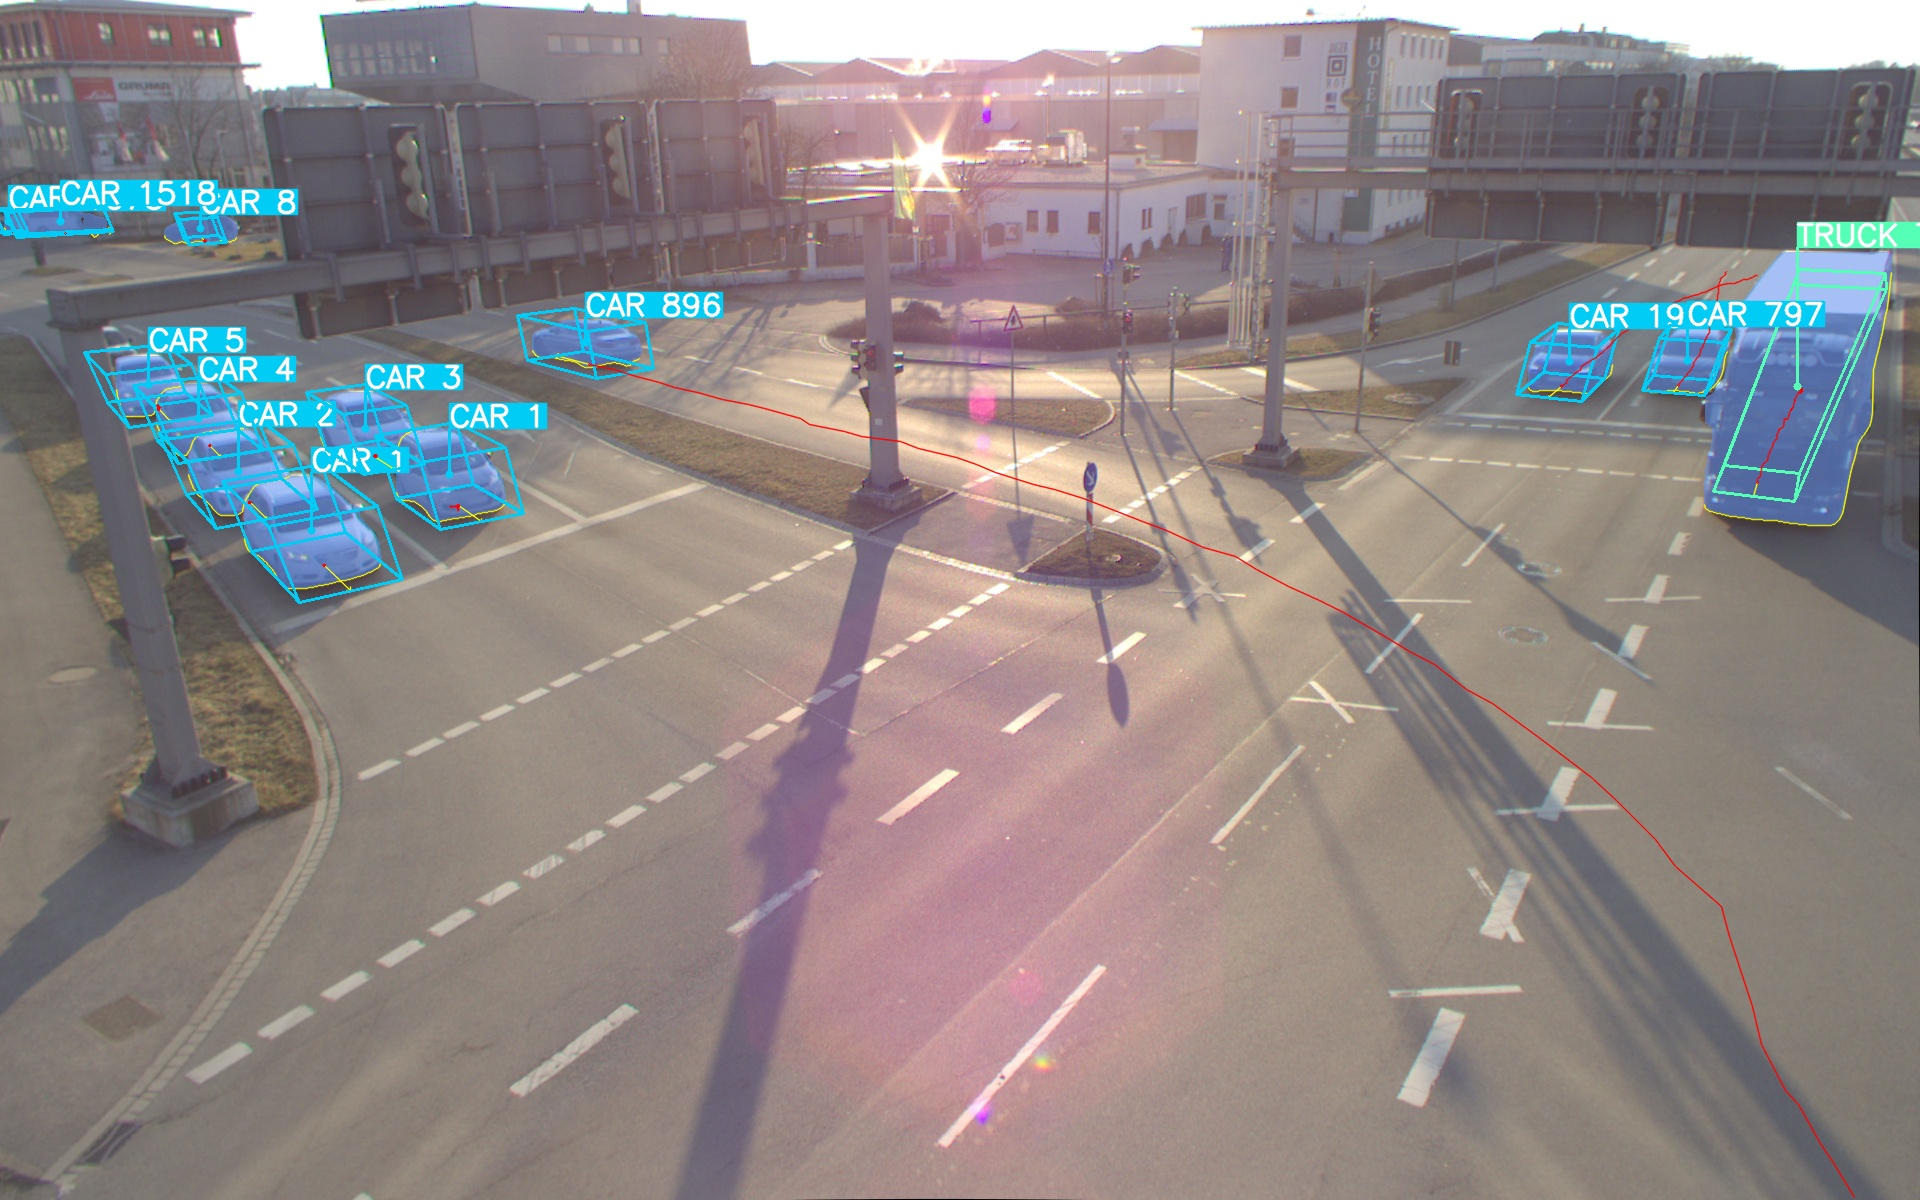
\includegraphics[width=0.499\linewidth]{
        figures/selection/1646667323-129810658-s110-camera-basler-south2-8mm}
    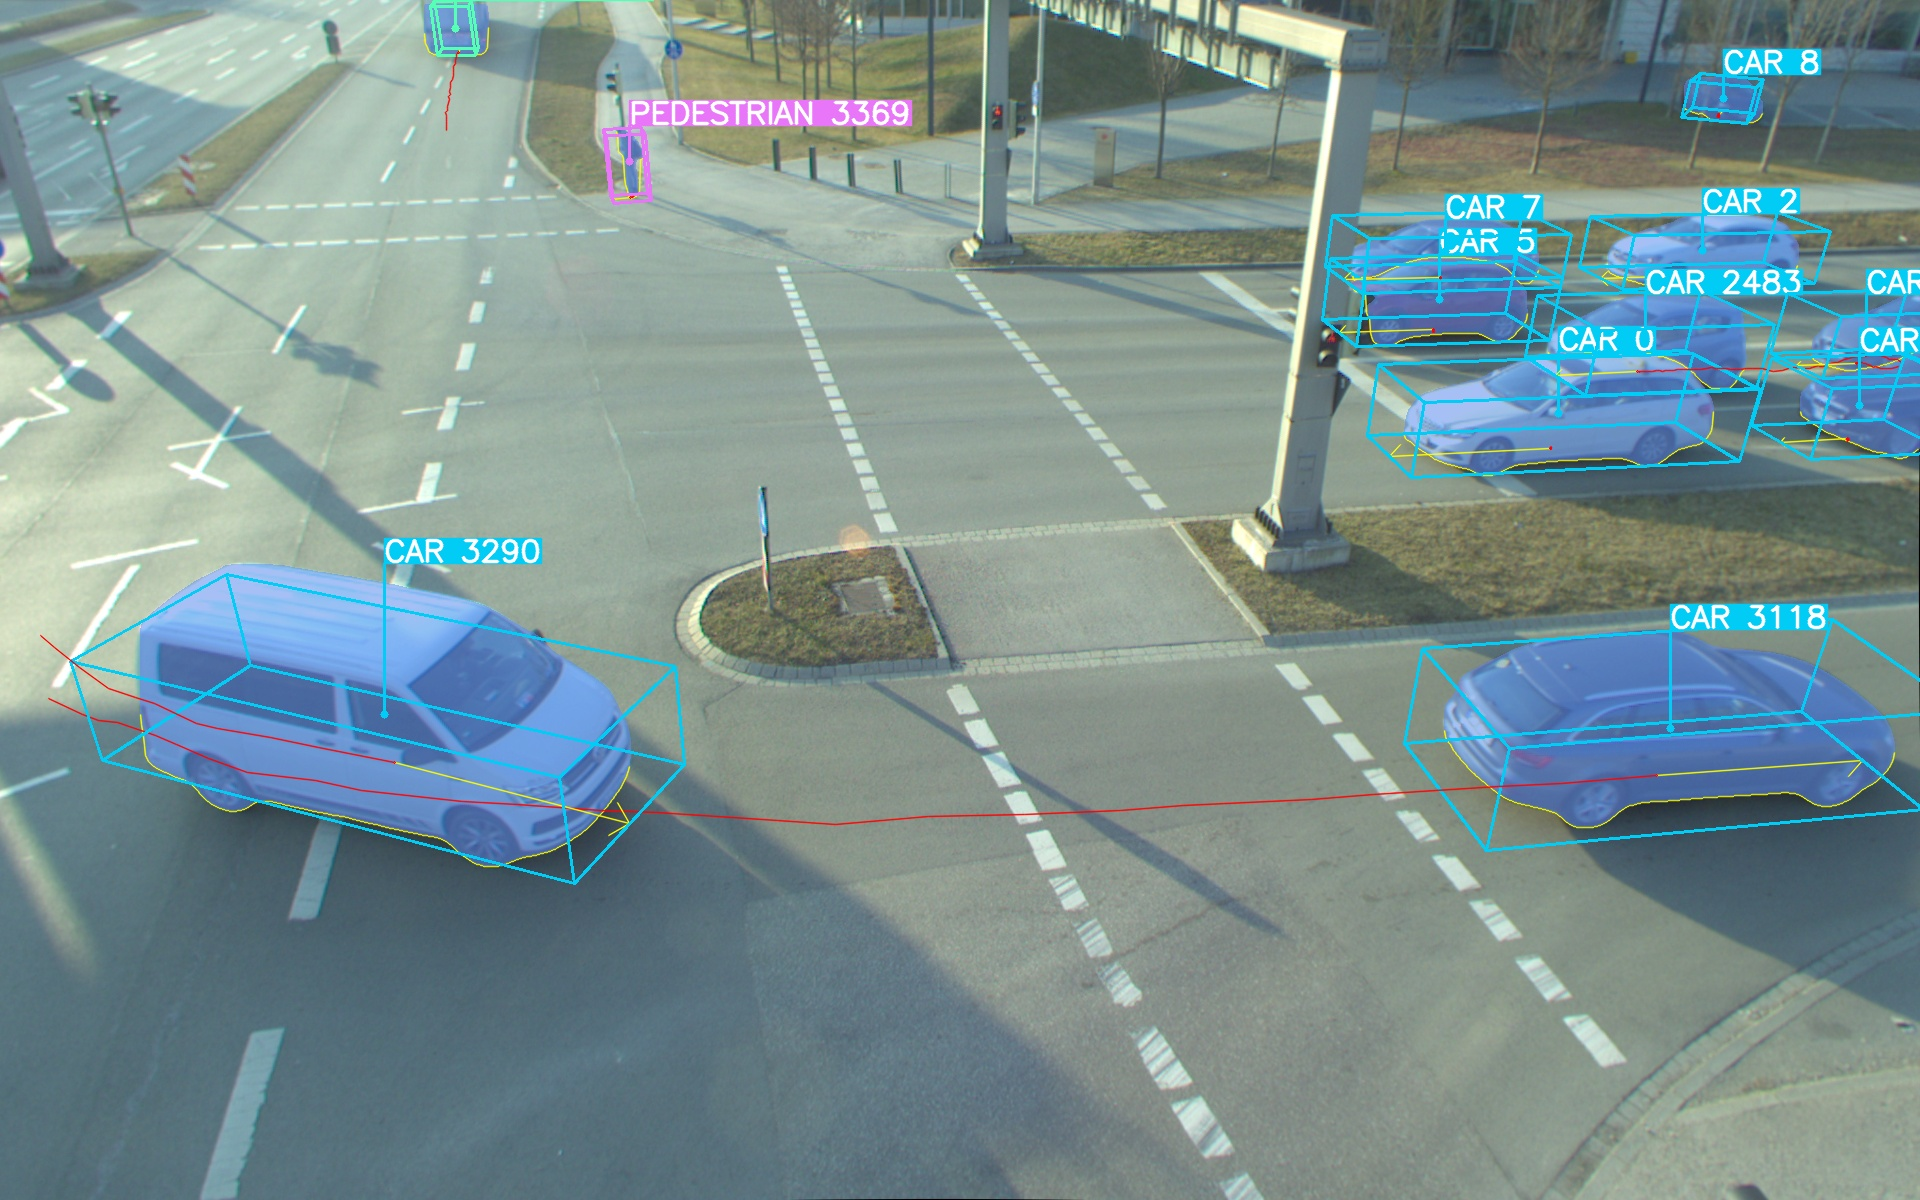
\includegraphics[width=0.499\linewidth]{
        figures/selection/1646667339-058779966-s110-camera-basler-south1-8mm} \\
    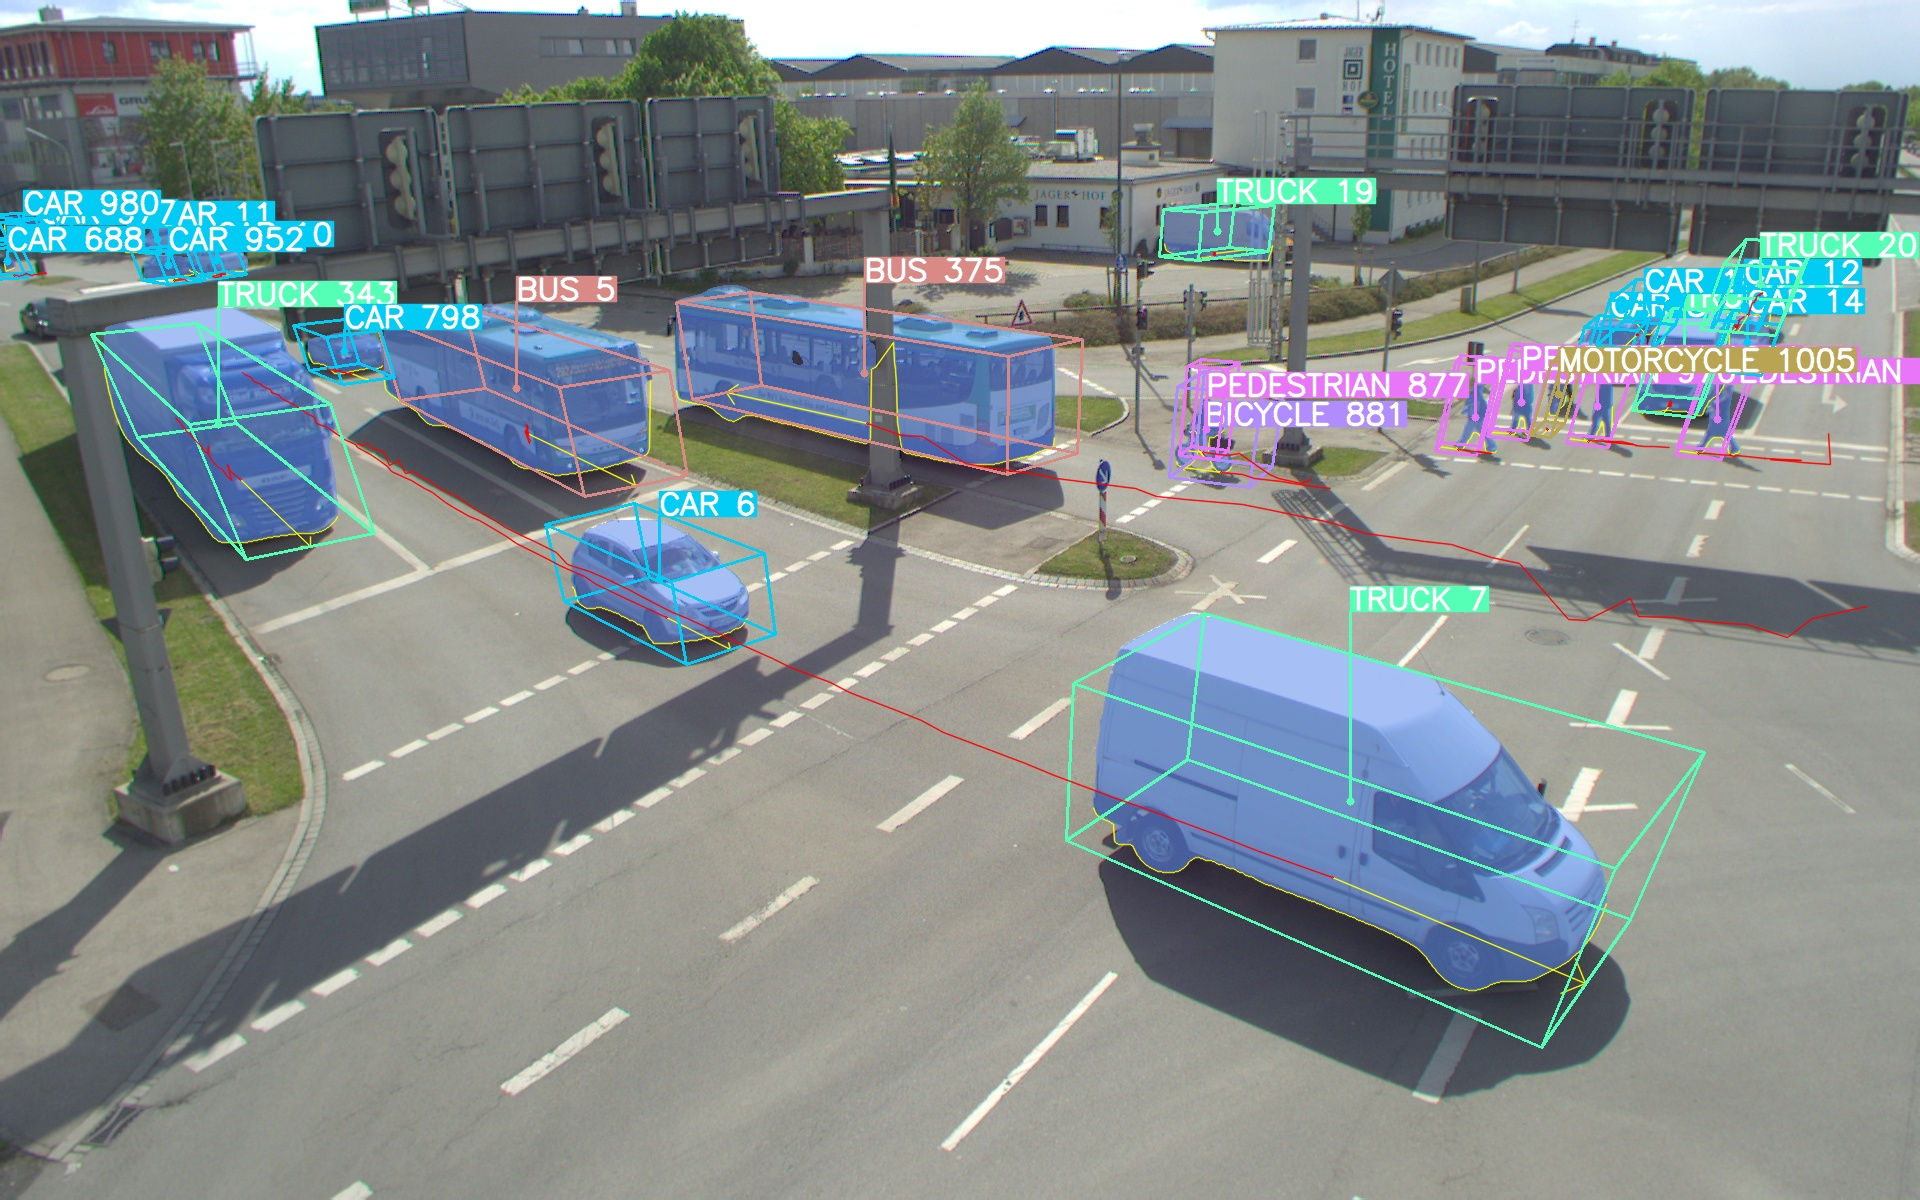
\includegraphics[width=0.499\linewidth]{
        figures/selection/1651673054-274505919-s110-camera-basler-south2-8mm}
    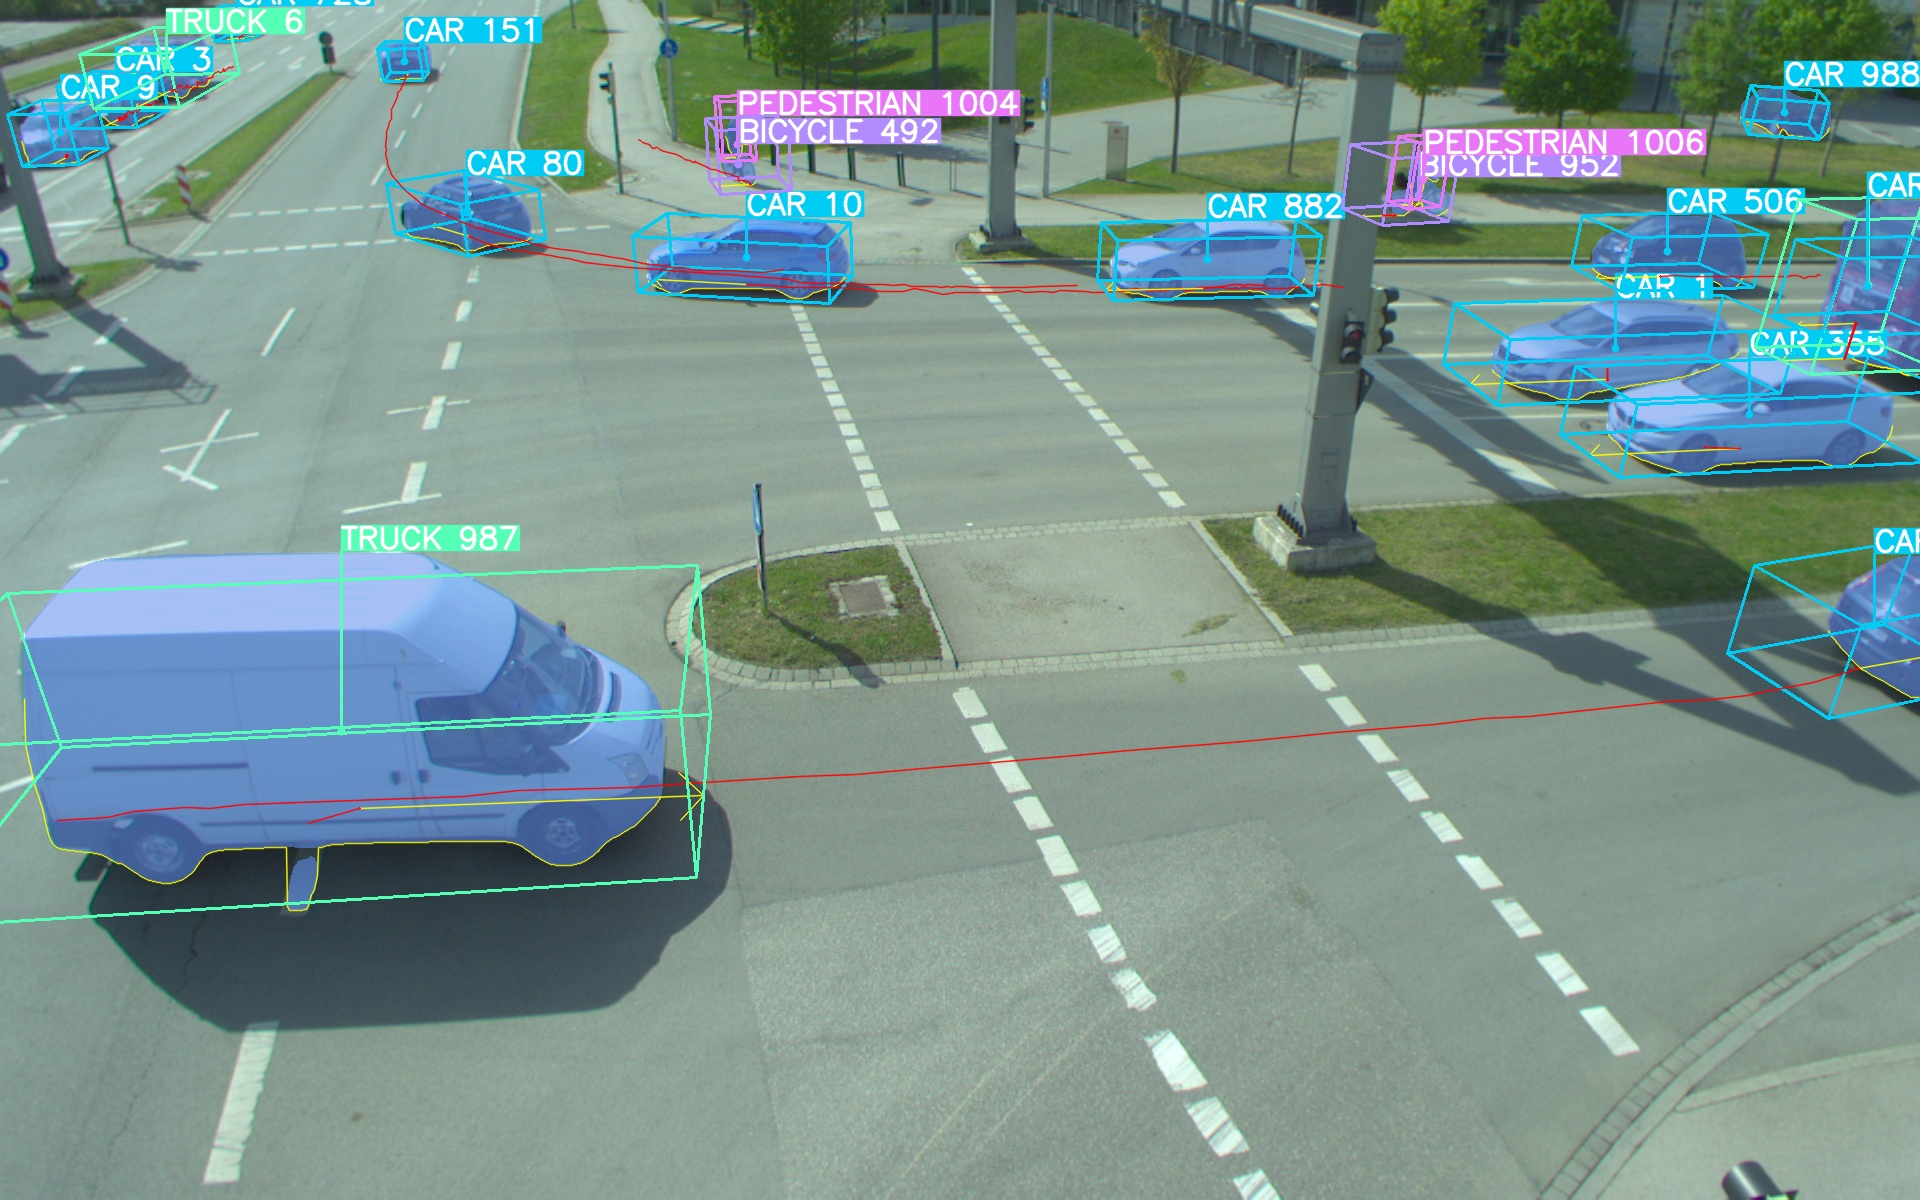
\includegraphics[width=0.499\linewidth]{
        figures/selection/1651673056-492970825-s110-camera-basler-south1-8mm}
    \caption{Hand-picked frames to showcase the qualitative performance of our implemented monocular 3D object detector during daytime.}
    \label{fig:qualitative-results-day}
\end{figure}

First off, Figure~\ref{fig:qualitative-results-day} shows representative frames with predicted vehicle bounding boxes, where the implemented system performs quite well.
The frames in the left column are from the South-2 camera, which has a greater detection range, as it is angled more towards the horizon.
The two frames for this camera show that the implemented system can correctly detect the 3D shapes of many overlapping vehicles, which are oriented opposed or perpendicular to each other.
The top-left frame showcases the good performance of the screen-space \textit{SORT} tracker, which tracks \texttt{CAR 896} throughout its whole left turn.
The bottom-left image shows the usefulness of the \textit{DBSCAN}-based bottom contour filter in the case of \texttt{BUS 375}.
The detection of this bus is split into two parts by the pole of the overhead gantry bridge.
This introduces a lot of noise into this detection's bottom contour, as highlighted in yellow.
However, the detected 3D bounding box is unaffected by this noise.
This frame also showcases the performance of our Vulnerable Road User (VRU) detection.
Both present pedestrians and bicycles in the image are correctly localized.

The frames in the right column are from the South-1 camera, which has a shorter detection range, as it is angled more towards the ground.
Both images in the right column again show generally good vehicle tracking and orientation estimation capabilities.

\begin{figure}[htb]
    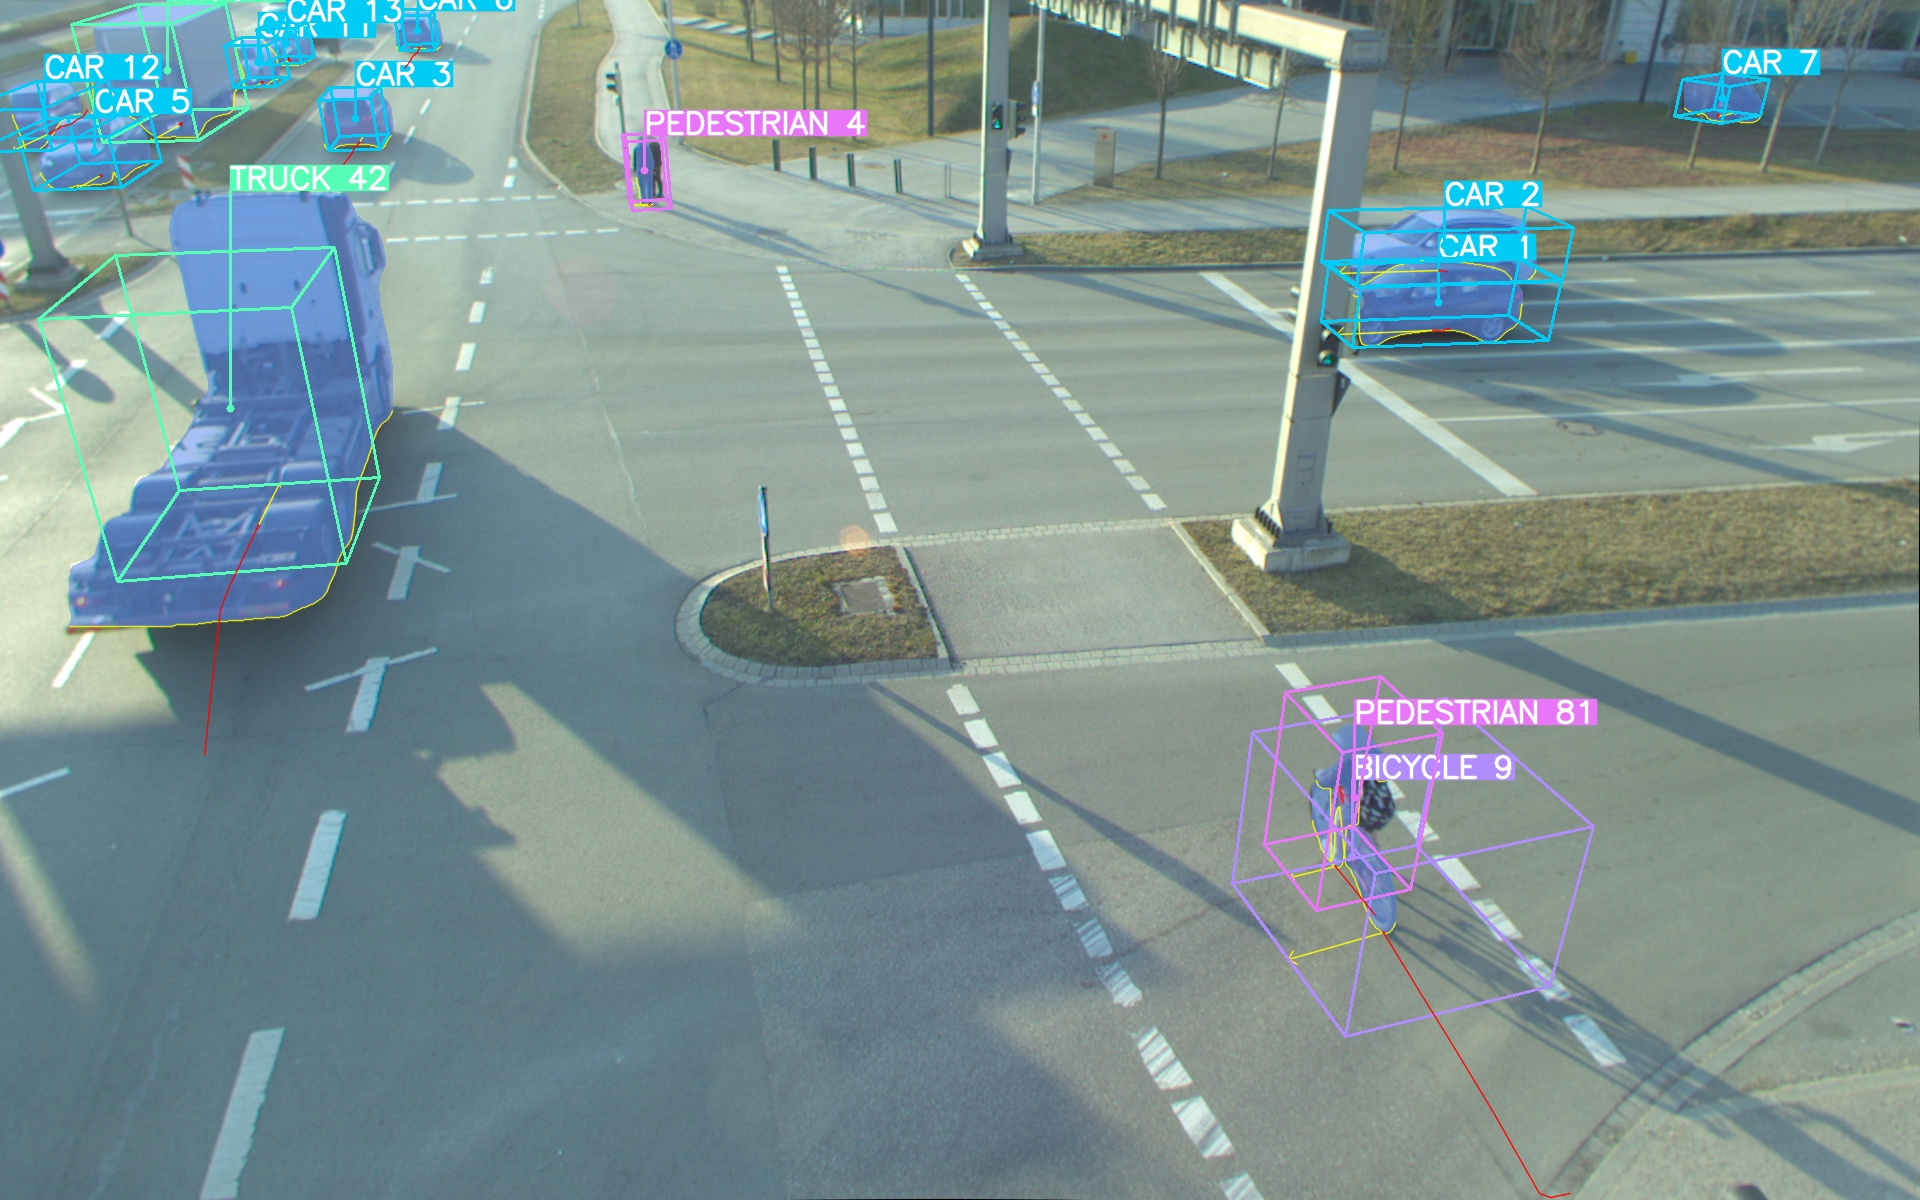
\includegraphics[width=0.499\linewidth]{
        figures/selection/1646667395-641065639-s110-camera-basler-south1-8mm}
    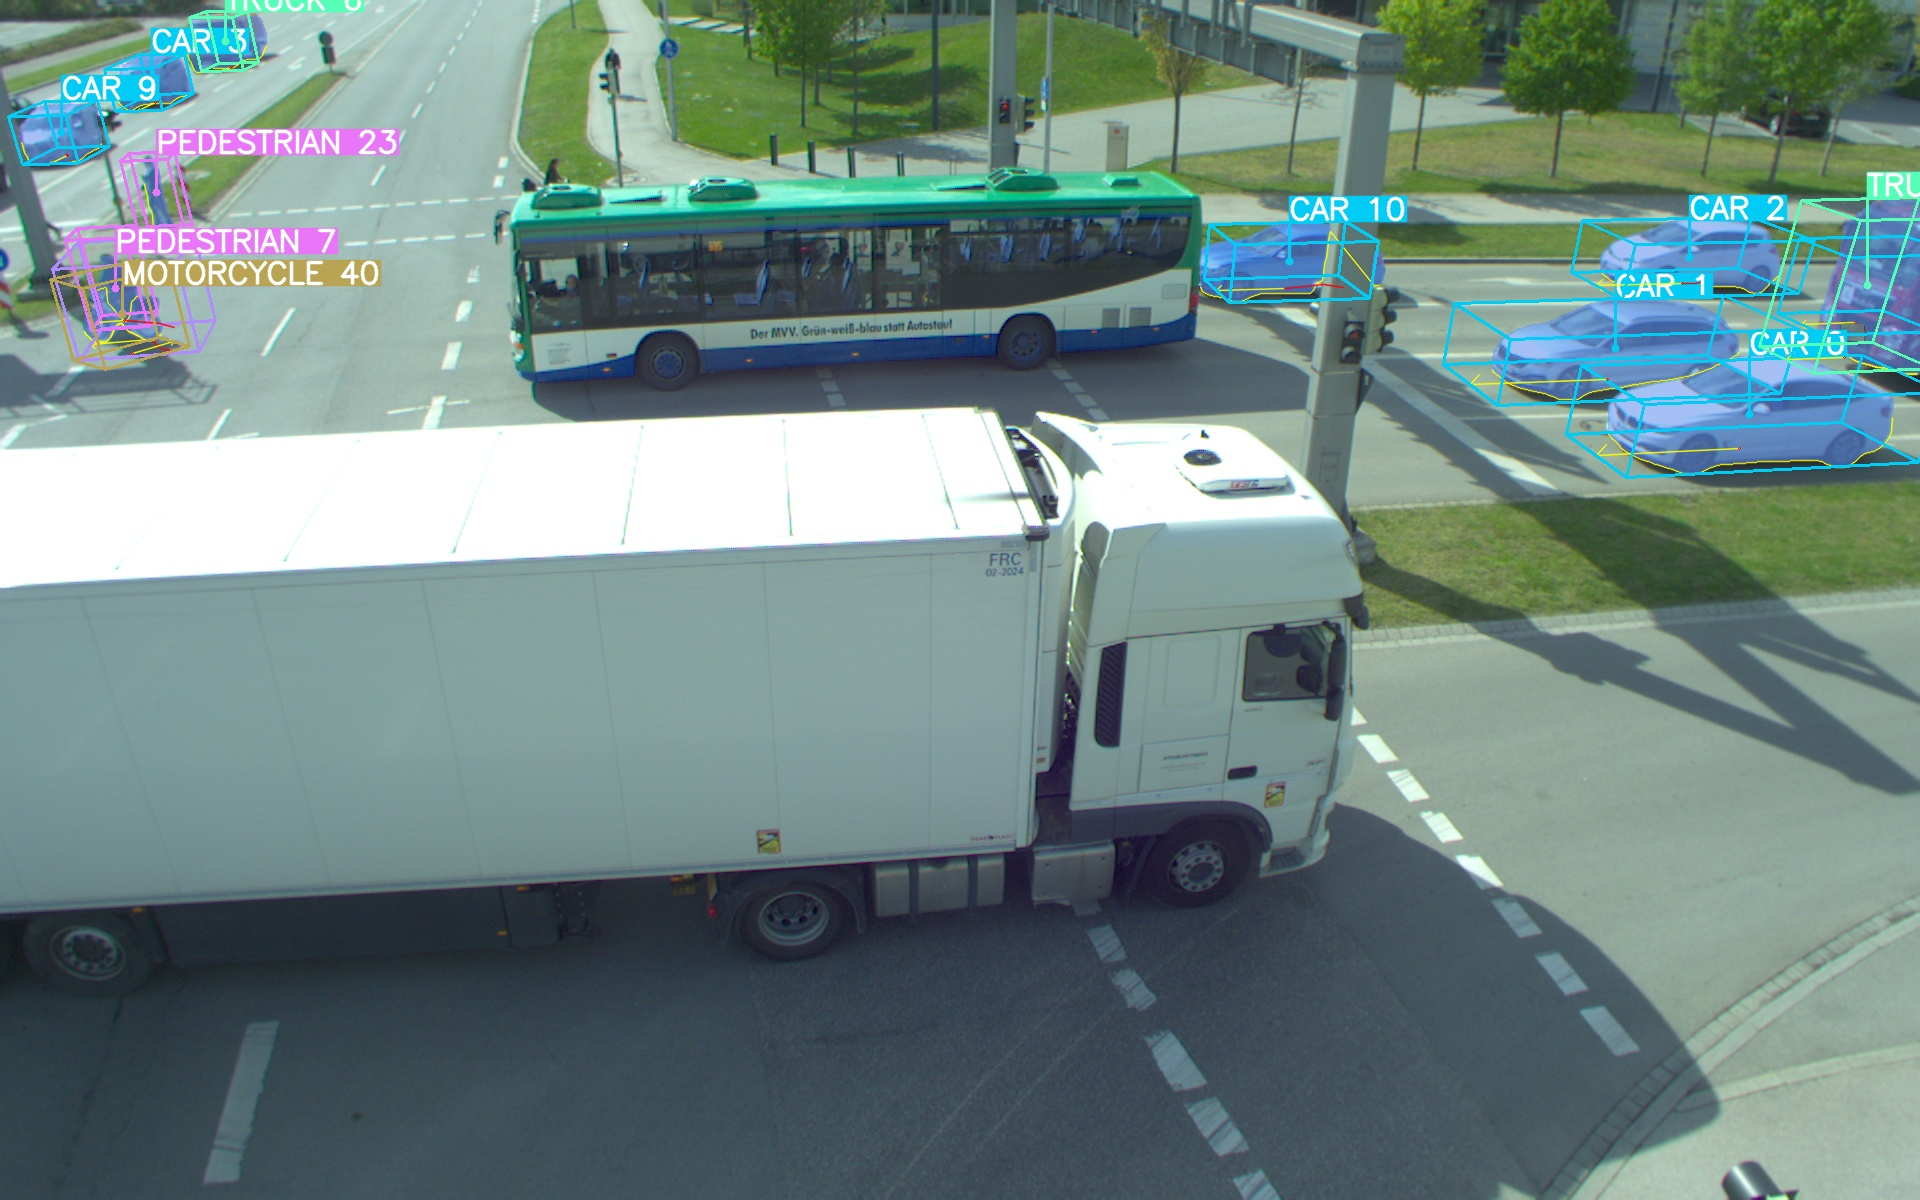
\includegraphics[width=0.499\linewidth]{
        figures/selection/1651673050-162472285-s110-camera-basler-south1-8mm}
    \caption{Selected frames to showcase problems of our implemented monocular 3D object detector.}
    \label{fig:qualitative-results-bad}
\end{figure}

Figure~\ref{fig:qualitative-results-bad} highlights particular weaknesses of the implemented monocular detector.
The image on the left highlights three problems.
First, the length estimation of \texttt{TRUCK 42} is bad, most likely due to over-eager bottom-contour filtering\footnote{This could be fixed by tweaking the $\epsilon$ (maximum point distance) and \texttt{min\_samples} (minimum cluster size) hyper-parameters for the \textit{DBSCAN} algorithm. We have set $\epsilon=0.5 m$ and $\mathtt{min\_samples}=5$}.
Second, only one of the two pedestrians is detected \textemdash \texttt{PEDESTRIAN 4} is standing next to another one.
Third, the system detects the rider of a bicycle as a separate entity, as in the case of \texttt{BICYCLE 9} and \texttt{PEDESTRIAN 81}.
This points to a need for more fine-tuned non-maximum suppression (NMS) of 3D detections.
The image on the right shows a single problem: Our detector (more specifically the used \textit{Yolov7} instance segmentation model) frequently has problems with detecting the instance masks of large objects near the camera.
In this case, both the big white truck in front of the camera, and the bus, which is a bit further away, are not detected.

\begin{figure}[htb]
    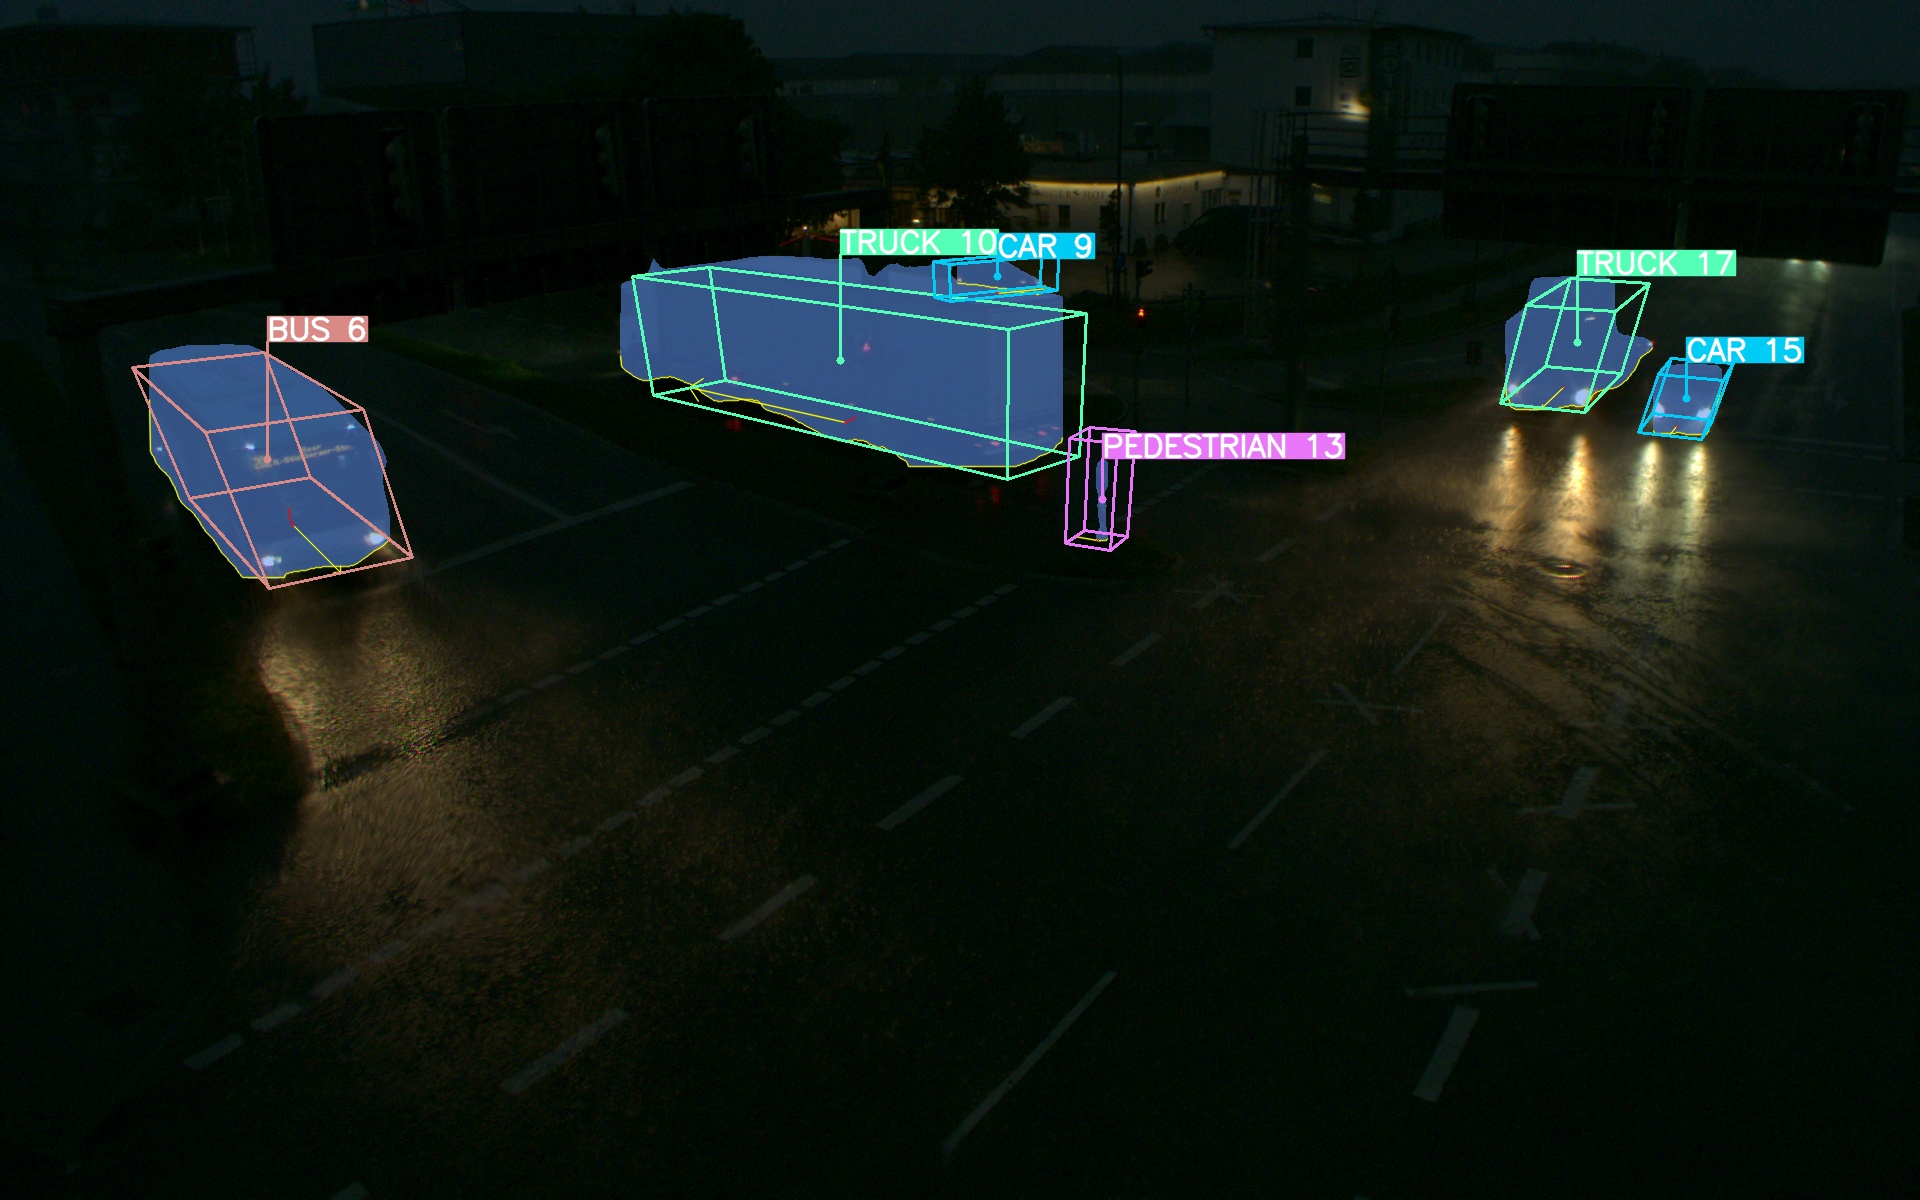
\includegraphics[width=0.499\linewidth]{
        figures/selection/1653330059-588901912-s110-camera-basler-south2-8mm}
    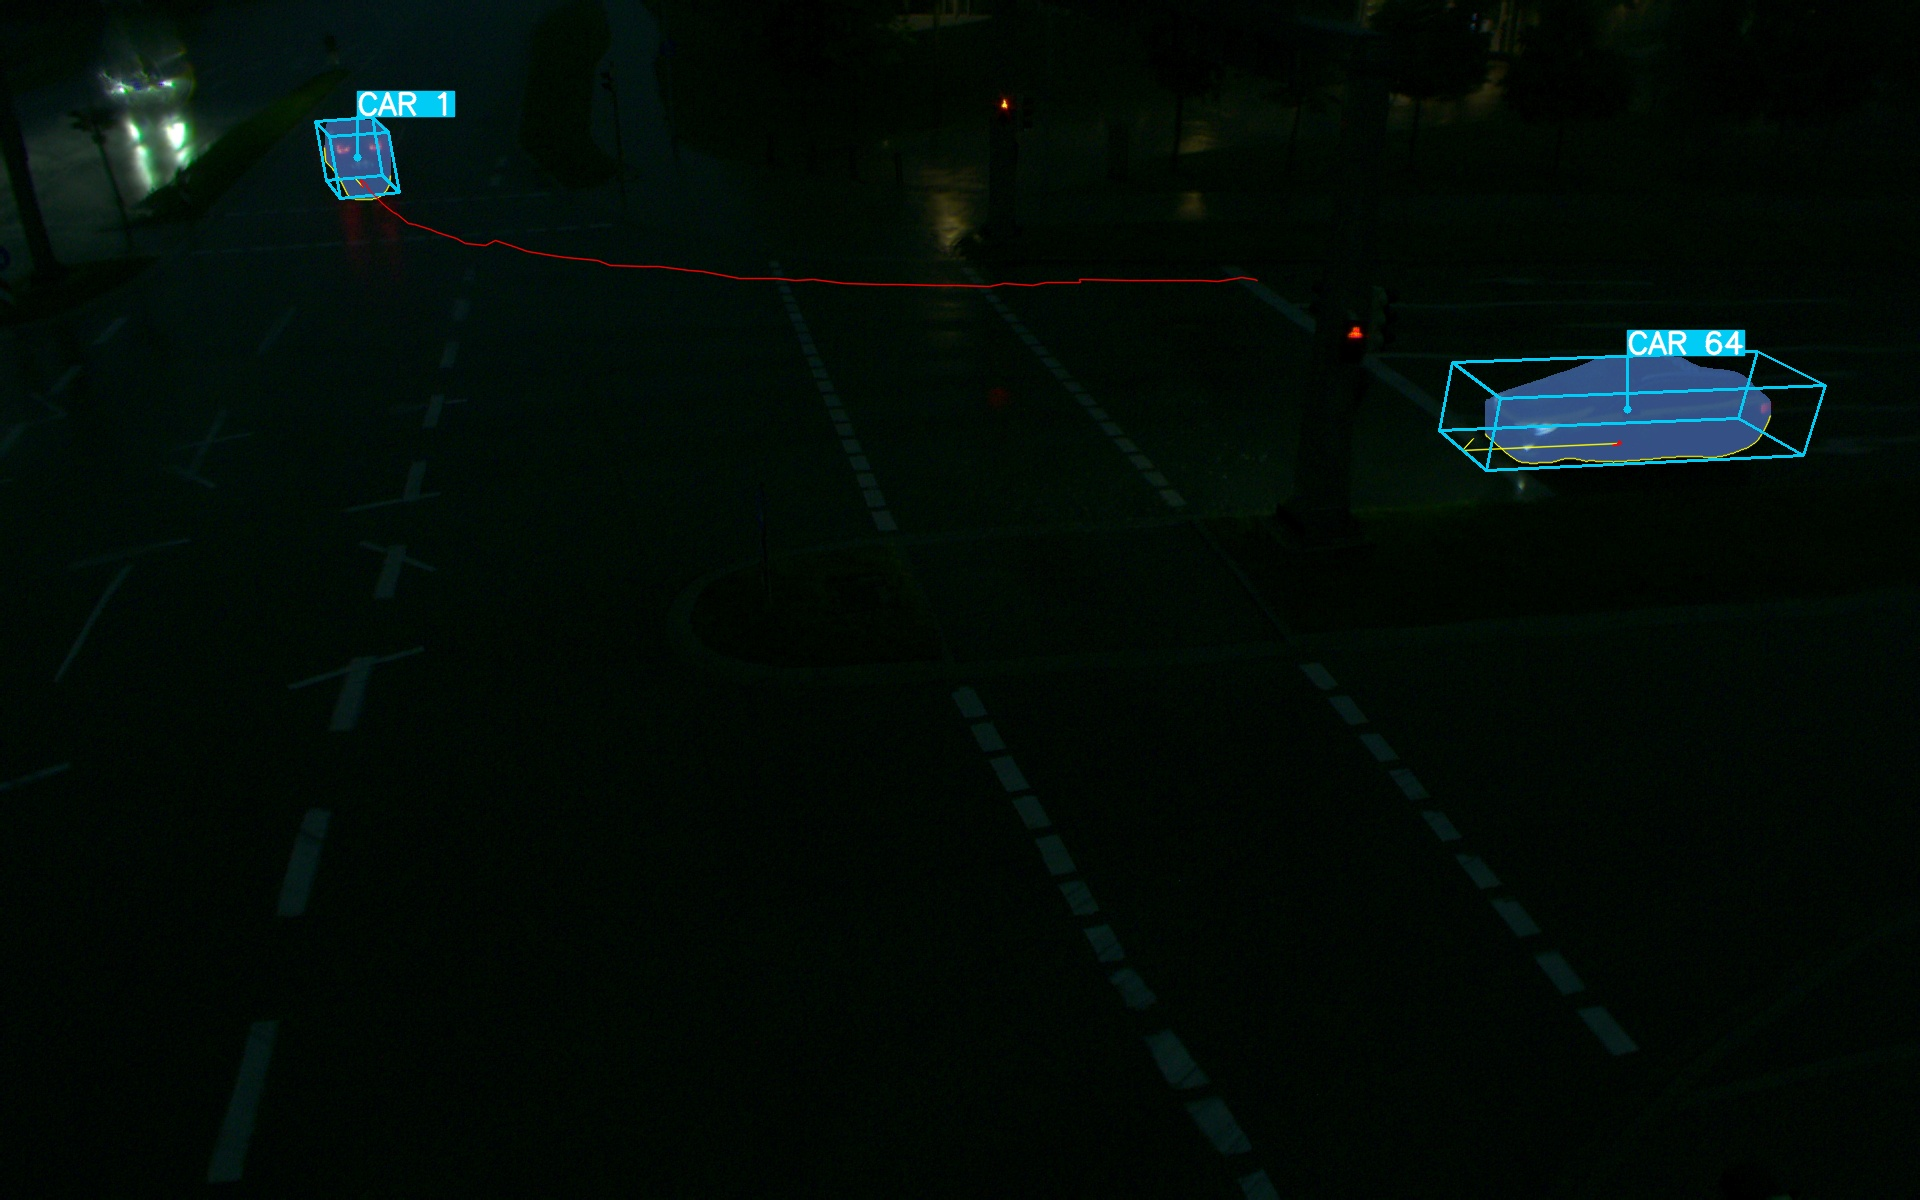
\includegraphics[width=0.499\linewidth]{
        figures/selection/1653330064-207615030-s110-camera-basler-south1-8mm}
    \caption{A selection of frames to showcase the qualitative performance of our implemented monocular 3D object detector at night.}
    \label{fig:qualitative-results-night}
\end{figure}

Finally, Figure~\ref{fig:qualitative-results-night} displays how the system performs at night.
Naturally, the detection performance of a system which is based on an RGB camera which operates in the human visible light spectrum will be worse at night, due to the reduced visibility.
However, the used \textit{Yolov7} instance segmentation model still works to some degree at night.
The predicted instance masks are generally noisier, and there are more false positives (such as \texttt{PEDESTRIAN 13}) and false negatives (such as the truck on the top-left in the right image).

% ----------------------------------------------------

\section{Runtime Performance}
\label{sec:performance}

The runtime performance of the monocular detection architecture is limited by the computational capabilities of the GPU. In our evaluation, we used an \textit{RTX-3090} GPU to assess the frame rates achieved by various models.
Table~\ref{tbl:gpu-performance} presents the frame-rates of the different models:

\begin{table*}[ht]
\centering
\caption{Model performance on \textit{RTX-3090} GPU}
\begin{tabular}{|l|c|}
\hline
\textbf{Model} & \textbf{Frame Rate (FPS)} \\
\hline
\textit{Yolact Edge ($550^2$ px)} & 60 \\
\textit{Yolov7 ($640^2$ px)} & 52 \\
\textit{Yolov7 ($1280^2$ px)} & 22 \\
\textit{Yolov7 ($1920^2$ px)} & 12 \\
\hline
\end{tabular}
\label{tbl:gpu-performance}
\end{table*}

As shown in Table~\ref{tbl:gpu-performance}, both \textit{Yolact Edge} and \textit{Yolov7-640} models achieve frame-rates between $55$ and $60$ FPS on the \textit{RTX-3090} GPU, indicating that they are suitable for real-time applications.
However, as the input resolution increases, the runtime performance of the models decreases.
For instance, \textit{Yolov7-1280} achieves $22$~FPS, and \textit{Yolov7-1920} reaches only $12$~FPS.
This analysis highlights the importance of considering the GPU constraints when designing and implementing two-stage monocular 3D object detection models, particularly for real-time applications.

% ----------------------------------------------------

\section{Quantitative Evaluation Strategy}
\label{sec:quant}

For an objective understanding of the performance of our \textit{Mono3D} solution, we performed a thorough ablative quantitative evaluation.
For this purpose, we use the \textit{Providentia Intersection Scenario} dataset, as previously mentioned in the Introduction (see Chapter~\ref{sec:a9dataset}).
As stated, the dataset provides 3D LiDAR labels for two camera perspectives onto the urban \textit{S110} road intersections.
For each camera, four scenes of varying length (between $300$ and $1200$ frames) are available.
The combination of two camera perspectives and four scenes yields eight frame sequences on which we evaluate our detector.
For each frame sequence, the detector is run in different configurations to evaluate the effect of various design choices on the final performance.
The detector is configured along four major components:

\begin{enumerate}
    \item \textbf{Instance Segmentation}: In the first detector stage, we can employ the \textit{Yolact}~\cite{liu2021yolactedge} instance segmentation model (running on 550x550 input frames), or the \textit{YoloV7}~\cite{wang2022yolov7} detector in $640x640$, $1280x180$, or $1920x1920$~px resolution mode.\ We respectively designate these modes as $I^{550}_\text{YOL}$, $I^{640}_\text{Yv7}$, $I^{1280}_\text{Yv7}$, and $I^{1920}_\text{Yv7}$.
    \item \textbf{Tracking}: This component concerns the usage of \textit{SORT tracking}~\cite{bewley2016simple} in our detector.\ We can apply tracking in $2D$ screen-space to assist the LSF algorithm, or in $3D$ space to stabilize vehicle position estimates, or both in $2D$ and $3D$, or not at all.\ We respectively designate these modes as $T_{2D}$, $T_{3D}$, $T^{2D}_{3D}$, and $T_0$.
    \item \textbf{HD Map Usage}: In this aspect, we consider whether to use heading information from the HD map as an early input to the LSF algorithm, as a late single-position lookup correction, or not at all.\ These modes are designated as $M_\text{LSF}$, $M_1$ and $M_0$.
    \item \textbf{Filtering}: Finally, we can switch two crucial filters on or off:\ The \textit{DBSCAN}~\cite{schubert2017dbscan} bottom contour point filter, and the output vehicle size filter.\ These modes will be symbolized as $F_\text{Cont}$, $F_\text{Size}$, $F_\text{Cont}^\text{Size}$, or $F_0$ (if no filter is used).
\end{enumerate}

In summary, each detector configuration is some combination of $I$, $T$, $M$ and $F$.\ For example, $\left[I^{640}_\text{Yv7}T^{2D}_{3D}M_\text{LSF}F_\text{Size}\right]$ would be the detector running with $640x640$~px \textit{Yolov7} instance segmentation, both 2D and 3D tracking, L-Shape-Fitting Map Input, and vehicle size filtering (but no bottom-contour filtering).
The combinatorial expansion yields $192$ possible detector configurations, which are executed on each of the $8$ LiDAR-labeled camera frame sequences.
This results in $1536$ prediction sequences.

Furthermore, we evaluate the impact which emerges from the sensor delay between the camera and the LiDAR sensor frames.
This delay is roughly $18.54$~ms on average.
This synchronization error is important, because we evaluate the 3D camera detections on labeled LiDAR sensor measurements.
These LiDAR labels will contain an inherent offset towards the camera detections due to the synchronization error.
We check whether the error can be reduced by estimating the spatial velocity of the LiDAR detections using \textit{SORT}, and then correcting the label position based on the velocity and the known synchronization error time delta.

We evaluate both the time-shifted and the original LiDAR labels with each prediction sequence.
We call these two label modes $L_0$ (original) and $L_{\uparrow}$ (shifted).
The label mode is appended to the detector configuration combination.
For each of the 3072 sequence-detector-label combinations and each road user class, we calculate the following metrics:

\begin{enumerate}
    \item The average orientation error \textbf{(AOE)} ($=\text{TP}_0$).
    \item The average translation error \textbf{(ATE)} ($=\text{TP}_1$.
    \item The average length error \textbf{(ALE)} ($=\text{TP}_2$).
    \item The average width error \textbf{(AWE)} ($=\text{TP}_3$).
    \item The average height error \textbf{(AHE)} ($=\text{TP}_4$).
    \item The average precision at $10$\% minimum $\mathbf{IoU}_{3D}$ \textbf{(AP@10)}.
    \item The average 3D intersection-over-union ($\mathbf{IoU}_{3D}$)
\end{enumerate}

In the following, the values for these metrics are presented in relation to particular detector- and labeling-configurations.
To judge the overall performance of a configuration, we aggregate these metrics into a single \enquote{Providentia Detection Score} (\textit{PDS}), similar to the \textit{nuScenes Detection Score} (see Section~\ref{sec:evalmetrics}):

\[
    \text{PDS} = \frac{1}{10} \left[5 * \text{mAP} + \sum^5_{k=1}(1-\text{min}(1, \text{mTP}_k))\right]
\]

The score is calculated for each configuration, by averaging the per-class metrics of the configuration across all perspectives of all dataset scenes.
A chart of all calculated Scores is shown in Figure~\ref{fig:all-scores}.
We consider the following object classes: \texttt{CAR}, \texttt{BUS}, \texttt{TRUCK}, \texttt{MOTORCYCLE}, \texttt{BICYCLE}, \texttt{PEDESTRIAN}.
Additionally, the A9 dataset contains annotations for \texttt{VAN}, \texttt{EMERGENCY\_VEHICLE}, \texttt{TRAILER} and \texttt{OTHER}.
However, these categories are not supported by our instance segmentation models, which will usually label these special vehicles as trucks or cars.
To gain a better understanding of our model's raw shape-estimation performance, we also evaluate using the \texttt{VEHICLE} super-class.
With the super-class, a \texttt{VAN} labeled as a \texttt{TRUCK} will still be considered as a True Positive detection.
Note that we skip the AOE metric for the pedestrians and bicycles, as we do not attempt to estimate their heading.

% ----------------------------------------------------

\section{Overall Quantitative Results}
\label{sec:baseline}

\begin{figure}[htb]
    
        \begin{tikzpicture}
        \begin{axis}[
            clip=false,
            ybar,
            width=\textwidth,
            height=0.4\textwidth,
            bar width=0.1pt,
            ylabel={Score},
            ymin=10, ymax=50,
            xtick=\empty,
            xticklabels={},
            enlarge x limits={abs=1pt},
        ]        
        
            \addplot [draw=blue, fill=none] table [x=xpos, y=yvalue, col sep=comma]{charts/overall.tex.blue.dat};
            \draw[black, thin, -latex]([xshift=0.1pt]axis cs:1,10) -- ++(axis direction cs:0,-8)node[below, font=\tiny, anchor=north west, outer sep=0] {\textbf{Model}: $\left[I^{550}_\text{YOL}T^{2D}_{3D}M_1F_0L_{\uparrow}\right]$: $13.58$};
\draw[black, thin, -latex]([xshift=0.1pt]axis cs:12,10) -- ++(axis direction cs:0,-3)node[below, font=\tiny, anchor=north west, outer sep=0] {\textbf{Model}: $\left[I^{550}_\text{YOL}T_0M_0F_0L_0\right]$: $17.78$};
\draw[black, thin, -latex]([xshift=0.1pt]axis cs:384,10) -- ++(axis direction cs:0,-3)node[below, font=\tiny, anchor=north east, outer sep=0] {\textbf{Model}: $\left[I^{1920}_\text{Yv7}T_{2D}M_\text{LSF}F_\text{Cont}^\text{Size}L_{\uparrow}\right]$: $40.17$};

        \end{axis}
        \end{tikzpicture}
        
    \caption{Overview for the \textit{Providentia Detection Score (PDS)} values of all possible 384 detector configuration-label combinations, with arrows pointing out the best, baseline, and worst combination.}
    \label{fig:all-scores}
\end{figure}

To establish the veracity of our score metric, we plotted the score values for all possible $384$ detector configuration-label combinations into a single chart.
This plot is shown in Figure~\ref{fig:all-scores}.
In this plot, the Scores of the worst-performing- ($\left[I^{550}_\text{YOL}T^{2D}_{3D}M_1F_0L_{\uparrow}\right]$), baseline- ( $\left[I^{550}_\text{YOL}T_0M_0F_0L_0\right]$), and best-performing ($\left[I^{1920}_\text{Yv7}T_{2D}M_\text{LSF}F_\text{Cont}^\text{Size}L_{\uparrow}\right]$) model-configurations are also highlighted.
The baseline model works with pure L-Shape-Fitting that does not use any HD map, tracking, or bottom-contour/size filtering augmentations.
Table~\ref{tbl:baseline} shows the performance of this model in greater detail.
Of particular interest is the large AOE of $52.19\degree$.
This means, that the predicted orientation of bounding boxes in this model is  completely disconnected from the ground truth.
Picking a random orientation would yield the same result.

\begin{table*}[htbp]
    
        \centering
        \scalebox{0.91}{
        \begin{tabular}{|l|rrrrrr|rrr|}
\hline & \multicolumn{6}{l|}{\textbf{Model}: $\left[I^{550}_\text{YOL}T_0M_0F_0L_0\right]$} & \multicolumn{3}{l|}{\textbf{PDS}: $15.31\%$} \rule{0pt}{1.4em} \\[0.2em] 

            \hline
            \hline
            \textbf{Class} & \textbf{AOE} & \textbf{ATE} & \textbf{AWE} & \textbf{ALE} & \textbf{AHE} & $\mathbf{IoU}_{3D}$ & \textbf{Precision} & \textbf{Recall} & \textbf{AP}{@}10 \\ 

            \hline
            Car & $57.39\degree$ & $1.10\nobreak\hspace{{.16667em plus .08333em}}m$ & $0.49\nobreak\hspace{{.16667em plus .08333em}}m$ & $1.03\nobreak\hspace{{.16667em plus .08333em}}m$ & $0.69\nobreak\hspace{{.16667em plus .08333em}}m$ & $21.80\%$ & $47.60\%$ & $40.57\%$ & $46.85\%$ \\ 
Truck & $34.61\degree$ & $2.17\nobreak\hspace{{.16667em plus .08333em}}m$ & $0.77\nobreak\hspace{{.16667em plus .08333em}}m$ & $4.15\nobreak\hspace{{.16667em plus .08333em}}m$ & $1.31\nobreak\hspace{{.16667em plus .08333em}}m$ & $20.31\%$ & $3.55\%$ & $1.67\%$ & $2.86\%$ \\ 
Motorcycle & $71.98\degree$ & $0.63\nobreak\hspace{{.16667em plus .08333em}}m$ & $0.76\nobreak\hspace{{.16667em plus .08333em}}m$ & $1.31\nobreak\hspace{{.16667em plus .08333em}}m$ & $0.13\nobreak\hspace{{.16667em plus .08333em}}m$ & $14.72\%$ & $31.14\%$ & $22.98\%$ & $30.68\%$ \\ 
Bus & $44.76\degree$ & $1.85\nobreak\hspace{{.16667em plus .08333em}}m$ & $1.47\nobreak\hspace{{.16667em plus .08333em}}m$ & $3.07\nobreak\hspace{{.16667em plus .08333em}}m$ & $1.55\nobreak\hspace{{.16667em plus .08333em}}m$ & $22.47\%$ & $17.47\%$ & $10.51\%$ & $16.19\%$ \\ 
Pedestrian & \textemdash & $0.38\nobreak\hspace{{.16667em plus .08333em}}m$ & $0.25\nobreak\hspace{{.16667em plus .08333em}}m$ & $0.18\nobreak\hspace{{.16667em plus .08333em}}m$ & $0.07\nobreak\hspace{{.16667em plus .08333em}}m$ & $21.62\%$ & $0.88\%$ & $0.10\%$ & $0.65\%$ \\ 
Bicycle & \textemdash & $0.34\nobreak\hspace{{.16667em plus .08333em}}m$ & $0.65\nobreak\hspace{{.16667em plus .08333em}}m$ & $0.46\nobreak\hspace{{.16667em plus .08333em}}m$ & $0.10\nobreak\hspace{{.16667em plus .08333em}}m$ & $20.46\%$ & $0.92\%$ & $0.17\%$ & $0.67\%$ \\ 

\hline
\textbf{Mean} & $\mathbf{52.19\degree}$ & $\mathbf{1.08\nobreak\hspace{{.16667em plus .08333em}}m}$ & $\mathbf{0.73\nobreak\hspace{{.16667em plus .08333em}}m}$ & $\mathbf{1.70\nobreak\hspace{{.16667em plus .08333em}}m}$ & $\mathbf{0.64\nobreak\hspace{{.16667em plus .08333em}}m}$ & $\mathbf{20.23\%}$ & $\mathbf{16.93\%}$ & $\mathbf{12.67\%}$ & $\mathbf{16.31\%}$ \\ 

            \hline
            
        \end{tabular}
        }
    \caption{Baseline model results.}
    \label{tbl:baseline}
\end{table*}

This stands in contrast to the performance metrics for the best-performing model, which are shown in Table~\ref{tbl:best}.
Additionally, Table~\ref{tbl:best-vehicles} shows the results for the best vehicle-only model.
In the following sections, we will discuss in detail how specific model configurations improve (or worsen) specific metrics for different road user classes.

\begin{table*}[htbp]
    
        \centering
        \scalebox{0.91}{
        \begin{tabular}{|l|rrrrrr|rrr|}
\hline & \multicolumn{6}{l|}{\textbf{Model}: $\left[I^{1920}_\text{Yv7}T_{2D}M_\text{LSF}F_\text{Cont}^\text{Size}L_{\uparrow}\right]$} & \multicolumn{3}{l|}{\textbf{Score}: $40.29\%$ $({\scriptstyle\color{TUMGreen}+24.98\%})$} \rule{0pt}{1.4em} \\[0.2em] 

            \hline
            \hline
            \textbf{Class} & \textbf{AOE} & \textbf{ATE} & \textbf{AWE} & \textbf{ALE} & \textbf{AHE} & $\mathbf{IoU}_{3D}$ & \textbf{Precision} & \textbf{Recall} & \textbf{AP}{@}10 \\ 

            \hline
            Car & $3.13\degree$ & $0.85m$ & $0.25m$ & $0.89m$ & $0.35m$ & $39.19\%$ & $72.76\%$ & $73.19\%$ & $72.26\%$ \\ 
Truck & $4.16\degree$ & $1.69m$ & $0.62m$ & $2.52m$ & $0.58m$ & $17.67\%$ & $23.47\%$ & $28.83\%$ & $22.84\%$ \\ 
Motorcycle & $3.85\degree$ & $0.78m$ & $0.31m$ & $0.63m$ & $0.14m$ & $26.91\%$ & $34.22\%$ & $30.43\%$ & $33.88\%$ \\ 
Bus & $10.35\degree$ & $1.15m$ & $0.55m$ & $2.93m$ & $1.08m$ & $33.55\%$ & $51.71\%$ & $35.50\%$ & $50.74\%$ \\ 
Pedestrian & \textemdash & $0.38m$ & $0.28m$ & $0.20m$ & $0.07m$ & $32.26\%$ & $20.84\%$ & $13.55\%$ & $20.45\%$ \\ 
Bicycle & \textemdash & $0.56m$ & $1.22m$ & $0.69m$ & $0.08m$ & $21.99\%$ & $33.75\%$ & $35.33\%$ & $33.49\%$ \\ 

\hline
\textbf{Mean} & $\mathbf{5.37\degree}$ & $\mathbf{0.90m}$ & $\mathbf{0.54m}$ & $\mathbf{1.31m}$ & $\mathbf{0.38m}$ & $\mathbf{28.59\%}$ & $\mathbf{39.46\%}$ & $\mathbf{36.14\%}$ & $\mathbf{38.94\%}$ \\ 
$\Delta$ {Baseline} & ${\scriptstyle\color{TUMGreen}-46.81\degree}$ & ${\scriptstyle\color{TUMGreen}-0.18m}$ & ${\scriptstyle\color{TUMGreen}-0.19m}$ & ${\scriptstyle\color{TUMGreen}-0.39m}$ & ${\scriptstyle\color{TUMGreen}-0.26m}$ & ${\scriptstyle\color{TUMGreen}+8.36\%}$ & ${\scriptstyle\color{TUMGreen}+22.53\%}$ & ${\scriptstyle\color{TUMGreen}+23.47\%}$ & ${\scriptstyle\color{TUMGreen}+22.63\%}$ \\ 

            \hline
            
        \end{tabular}
        }
    \caption{Best model results, with improvements towards the baseline highlighted in green for each metric.}
    \label{tbl:best}
\end{table*}

\begin{table*}[htbp]
    
        \centering
        \scalebox{0.91}{
        \begin{tabular}{|l|rrrrrr|rrr|}
\hline & \multicolumn{6}{l|}{\textbf{Model}: $\left[I^{1920}_\text{Yv7}T_{2D}M_\text{LSF}F_\text{Cont}^\text{Size}L_{\uparrow}\right]$} & \multicolumn{3}{l|}{\textbf{Score}: $50.07\%$ $({\scriptstyle\color{TUMGreen}+26.40\%})$} \rule{0pt}{1.4em} \\[0.2em] 

            \hline
            \hline
            \textbf{Class} & \textbf{AOE} & \textbf{ATE} & \textbf{AWE} & \textbf{ALE} & \textbf{AHE} & $\mathbf{IoU}_{3D}$ & \textbf{Precision} & \textbf{Recall} & \textbf{AP}{@}10 \\ 

            \hline
            Vehicle & $3.47\degree$ & $0.96m$ & $0.33m$ & $1.30m$ & $0.44m$ & $36.79\%$ & $56.72\%$ & $48.18\%$ & $55.90\%$ \\ 
$\Delta$ {Baseline} & ${\scriptstyle\color{TUMGreen}-52.79\degree}$ & ${\scriptstyle\color{TUMGreen}-0.25m}$ & ${\scriptstyle\color{TUMGreen}-0.35m}$ & ${\scriptstyle\color{TUMGreen}-0.27m}$ & ${\scriptstyle\color{TUMGreen}-0.36m}$ & ${\scriptstyle\color{TUMGreen}+15.41\%}$ & ${\scriptstyle\color{TUMGreen}+19.22\%}$ & ${\scriptstyle\color{TUMGreen}+21.32\%}$ & ${\scriptstyle\color{TUMGreen}+19.36\%}$ \\ 

            \hline
            
        \end{tabular}
        }
    \caption{Best model results focusing on the \texttt{Vehicle} super-category, with improvements towards the vehicle-only baseline highlighted in green for each metric.}
    \label{tbl:best-vehicles}
\end{table*}

% ----------------------------------------------------

\section{Influence of Late HD Map Lookup}
\label{sec:impactlatemap}

In this section, we present the evaluation of the \enquote{Late HD Map Lookup} technique, a simpler alternative to the \enquote{early} HD map lookup.
As mentioned in Section~\ref{sec:hdmaplate}, this approach has several drawbacks which are expected to negatively impact the system's performance.
The purpose of this evaluation is to provide a clear understanding of the limitations and consequences of using the late lookup approach.
This was the first approach we tried to improve upon the baseline detector.
The metrics of a Yolact-based detector which simply adds late HD map-lookup-based heading correction are presented in Table~\ref{tbl:late-lookup-results}.

\begin{table*}[htbp]
    
        \centering
        \scalebox{0.91}{
        \begin{tabular}{|l|rrrrrr|rrr|}
\hline & \multicolumn{6}{l|}{\textbf{Model}: $\left[I^{550}_\text{YOL}T_0M_1F_0L_0\right]$} & \multicolumn{3}{l|}{\textbf{Score}: $19.56\%$ $({\scriptstyle\color{TUMGreen}+4.25\%})$} \rule{0pt}{1.4em} \\[0.2em] 

            \hline
            \hline
            \textbf{Class} & \textbf{AOE} & \textbf{ATE} & \textbf{AWE} & \textbf{ALE} & \textbf{AHE} & $\mathbf{IoU}_{3D}$ & \textbf{Precision} & \textbf{Recall} & \textbf{AP}{@}10 \\ 

            \hline
            Car & $45.15\degree$ & $1.13m$ & $0.48m$ & $1.10m$ & $0.68m$ & $27.26\%$ & $46.89\%$ & $39.65\%$ & $46.12\%$ \\ 
Truck & $50.81\degree$ & $2.47m$ & $0.88m$ & $4.90m$ & $1.18m$ & $18.93\%$ & $4.27\%$ & $2.59\%$ & $3.55\%$ \\ 
Motorcycle & $13.04\degree$ & $0.40m$ & $0.49m$ & $0.95m$ & $0.05m$ & $11.14\%$ & $36.05\%$ & $27.21\%$ & $35.77\%$ \\ 
Bus & $36.76\degree$ & $1.81m$ & $1.32m$ & $3.63m$ & $1.62m$ & $25.44\%$ & $21.03\%$ & $14.67\%$ & $19.80\%$ \\ 
Pedestrian & \textemdash & $0.38m$ & $0.25m$ & $0.18m$ & $0.07m$ & $21.52\%$ & $0.88\%$ & $0.10\%$ & $0.65\%$ \\ 
Bicycle & \textemdash & $0.34m$ & $0.65m$ & $0.46m$ & $0.10m$ & $20.43\%$ & $0.92\%$ & $0.17\%$ & $0.67\%$ \\ 

\hline
\textbf{Mean} & $\mathbf{36.44\degree}$ & $\mathbf{1.09m}$ & $\mathbf{0.68m}$ & $\mathbf{1.87m}$ & $\mathbf{0.62m}$ & $\mathbf{20.78\%}$ & $\mathbf{18.34\%}$ & $\mathbf{14.07\%}$ & $\mathbf{17.76\%}$ \\ 
$\Delta$ {Baseline} & ${\scriptstyle\color{TUMGreen}-15.75\degree}$ & ${\scriptstyle\color{red}+0.01m}$ & ${\scriptstyle\color{TUMGreen}-0.05m}$ & ${\scriptstyle\color{red}+0.17m}$ & ${\scriptstyle\color{TUMGreen}-0.02m}$ & ${\scriptstyle\color{TUMGreen}+0.55\%}$ & ${\scriptstyle\color{TUMGreen}+1.41\%}$ & ${\scriptstyle\color{TUMGreen}+1.40\%}$ & ${\scriptstyle\color{TUMGreen}+1.44\%}$ \\ 

            \hline
            
        \end{tabular}
        }
    \caption{Results for the simplest possible late map lookup detector, with differences towards the baseline highlighted in red and green.}
    \label{tbl:late-lookup-results}
\end{table*}

One of the main issues with the late HD map lookup is that it takes place after the L-Shape-Fitting has already determined a heading value.
This means that the heading information from the HD map cannot be used to guide or correct the LSF-based size , leading to inaccuracies in the width and length estimation.
This is also shown in the results, as none of the size or translation metrics are significantly improved.

Another significant drawback of the late HD map lookup is that it discards a lot of the positional information from the ground truth sensor input.
By querying the HD map only for heading options at the predicted vehicle position, the system loses the ability to take advantage of the more accurate and granular bottom contour data from the sensor inputs.
This loss of information is reflected in the barely improved orientation error.

% ----------------------------------------------------

\section{Effects of YOLOv7 and Image Resolution}
\label{sec:impactyolov7}

\begin{table*}[htbp]
    
        \centering
        \scalebox{0.91}{
        \begin{tabular}{|l|rrrrrr|rrr|}
\hline & \multicolumn{6}{l|}{\textbf{Average Results Using Yolact-Edge}} & \multicolumn{3}{l|}{\textbf{Score}: $27.45\%$} \rule{0pt}{1.4em} \\[0.2em] 

            \hline
            \hline
            \textbf{Class} & \textbf{AOE} & \textbf{ATE} & \textbf{AWE} & \textbf{ALE} & \textbf{AHE} & $\mathbf{IoU}_{3D}$ & \textbf{Precision} & \textbf{Recall} & \textbf{AP}{@}10 \\ 

            \hline
            Vehicle & $32.92\degree$ & $1.05m$ & $0.48m$ & $1.52m$ & $0.62m$ & $30.66\%$ & $49.16\%$ & $39.74\%$ & $48.29\%$ \\ 
Car & $32.30\degree$ & $0.90m$ & $0.38m$ & $1.11m$ & $0.48m$ & $31.80\%$ & $59.97\%$ & $58.41\%$ & $59.36\%$ \\ 
Truck & $31.64\degree$ & $2.05m$ & $0.64m$ & $4.18m$ & $1.07m$ & $20.84\%$ & $12.31\%$ & $10.01\%$ & $11.80\%$ \\ 
Motorcycle & $35.79\degree$ & $0.60m$ & $0.31m$ & $0.46m$ & $0.12m$ & $19.16\%$ & $33.52\%$ & $24.69\%$ & $33.11\%$ \\ 
Bus & $31.22\degree$ & $1.53m$ & $0.94m$ & $3.00m$ & $1.42m$ & $27.55\%$ & $34.50\%$ & $23.45\%$ & $33.32\%$ \\ 
Pedestrian & $21.78\degree$ & $0.38m$ & $0.25m$ & $0.17m$ & $0.07m$ & $20.91\%$ & $0.85\%$ & $0.10\%$ & $0.63\%$ \\ 
Bicycle & $34.30\degree$ & $0.26m$ & $0.65m$ & $0.46m$ & $0.10m$ & $22.55\%$ & $0.92\%$ & $0.17\%$ & $0.67\%$ \\ 

\hline
\textbf{Mean} & $\mathbf{31.42\degree}$ & $\mathbf{0.97m}$ & $\mathbf{0.52m}$ & $\mathbf{1.56m}$ & $\mathbf{0.55m}$ & $\mathbf{24.78\%}$ & $\mathbf{27.32\%}$ & $\mathbf{22.37\%}$ & $\mathbf{26.74\%}$ \\ 

            \hline
            \hline & \multicolumn{6}{l|}{\textbf{Average Results Using Yolov7 (640x640)}} & \multicolumn{3}{l|}{\textbf{Score}: $28.80\%$ $({\scriptstyle\color{TUMGreen}+1.35})$} \rule{0pt}{1.4em} \\[0.2em] 

            \hline
            \hline
            \textbf{Class} & \textbf{AOE} & \textbf{ATE} & \textbf{AWE} & \textbf{ALE} & \textbf{AHE} & $\mathbf{IoU}_{3D}$ & \textbf{Precision} & \textbf{Recall} & \textbf{AP}{@}10 \\ 

            \hline
            Vehicle & $32.89\degree$ & $1.07m$ & $0.57m$ & $1.82m$ & $0.59m$ & $29.09\%$ & $48.00\%$ & $39.40\%$ & $47.11\%$ \\ 
Car & $32.09\degree$ & $0.88m$ & $0.44m$ & $1.16m$ & $0.39m$ & $30.52\%$ & $61.42\%$ & $59.80\%$ & $60.79\%$ \\ 
Truck & $28.94\degree$ & $2.17m$ & $0.89m$ & $4.85m$ & $0.84m$ & $15.67\%$ & $10.45\%$ & $10.86\%$ & $9.71\%$ \\ 
Motorcycle & $28.69\degree$ & $0.50m$ & $0.32m$ & $0.36m$ & $0.14m$ & $25.69\%$ & $36.73\%$ & $27.54\%$ & $36.27\%$ \\ 
Bus & $30.73\degree$ & $1.30m$ & $0.84m$ & $3.66m$ & $1.00m$ & $26.03\%$ & $35.27\%$ & $22.24\%$ & $34.24\%$ \\ 
Pedestrian & $29.90\degree$ & $0.33m$ & $0.22m$ & $0.17m$ & $0.07m$ & $24.41\%$ & $6.81\%$ & $1.23\%$ & $6.05\%$ \\ 
Bicycle & $47.01\degree$ & $0.52m$ & $1.09m$ & $0.62m$ & $0.10m$ & $27.09\%$ & $15.10\%$ & $6.40\%$ & $14.36\%$ \\ 

\hline
\textbf{Mean} & $\mathbf{32.89\degree}$ & $\mathbf{0.97m}$ & $\mathbf{0.62m}$ & $\mathbf{1.81m}$ & $\mathbf{0.45m}$ & $\mathbf{25.50\%}$ & $\mathbf{30.54\%}$ & $\mathbf{23.92\%}$ & $\mathbf{29.79\%}$ \\ 
$\Delta$ {Previous} & ${\scriptstyle\color{red}+1.47\degree}$ & ${\scriptstyle\color{TUMGreen}0.00m}$ & ${\scriptstyle\color{red}+0.10m}$ & ${\scriptstyle\color{red}+0.25m}$ & ${\scriptstyle\color{TUMGreen}-0.11m}$ & ${\scriptstyle\color{TUMGreen}+0.72\%}$ & ${\scriptstyle\color{TUMGreen}+3.22\%}$ & ${\scriptstyle\color{TUMGreen}+1.56\%}$ & ${\scriptstyle\color{TUMGreen}+3.05\%}$ \\ 

            \hline
            \hline & \multicolumn{6}{l|}{\textbf{Average Results Using Yolov7 (1280x1280)}} & \multicolumn{3}{l|}{\textbf{Score}: $30.64\%$ $({\scriptstyle\color{TUMGreen}+1.84})$} \rule{0pt}{1.4em} \\[0.2em] 

            \hline
            \hline
            \textbf{Class} & \textbf{AOE} & \textbf{ATE} & \textbf{AWE} & \textbf{ALE} & \textbf{AHE} & $\mathbf{IoU}_{3D}$ & \textbf{Precision} & \textbf{Recall} & \textbf{AP}{@}10 \\ 

            \hline
            Vehicle & $32.91\degree$ & $1.09m$ & $0.52m$ & $1.65m$ & $0.59m$ & $30.08\%$ & $48.22\%$ & $40.13\%$ & $47.27\%$ \\ 
Car & $32.67\degree$ & $0.90m$ & $0.38m$ & $1.03m$ & $0.45m$ & $31.42\%$ & $61.55\%$ & $60.01\%$ & $60.88\%$ \\ 
Truck & $31.03\degree$ & $2.16m$ & $0.85m$ & $4.58m$ & $0.73m$ & $19.03\%$ & $14.19\%$ & $15.08\%$ & $13.65\%$ \\ 
Motorcycle & $33.22\degree$ & $0.63m$ & $0.38m$ & $0.66m$ & $0.14m$ & $25.12\%$ & $36.84\%$ & $28.91\%$ & $36.43\%$ \\ 
Bus & $29.61\degree$ & $1.40m$ & $0.97m$ & $2.88m$ & $1.25m$ & $28.01\%$ & $44.14\%$ & $29.82\%$ & $43.21\%$ \\ 
Pedestrian & $23.90\degree$ & $0.26m$ & $0.22m$ & $0.17m$ & $0.06m$ & $28.98\%$ & $13.53\%$ & $7.38\%$ & $13.01\%$ \\ 
Bicycle & $40.91\degree$ & $0.66m$ & $1.20m$ & $0.64m$ & $0.08m$ & $21.87\%$ & $29.59\%$ & $32.15\%$ & $29.25\%$ \\ 

\hline
\textbf{Mean} & $\mathbf{32.04\degree}$ & $\mathbf{1.01m}$ & $\mathbf{0.64m}$ & $\mathbf{1.66m}$ & $\mathbf{0.47m}$ & $\mathbf{26.36\%}$ & $\mathbf{35.44\%}$ & $\mathbf{30.50\%}$ & $\mathbf{34.81\%}$ \\ 
$\Delta$ {Previous} & ${\scriptstyle\color{TUMGreen}-0.86\degree}$ & ${\scriptstyle\color{red}+0.05m}$ & ${\scriptstyle\color{red}+0.02m}$ & ${\scriptstyle\color{TUMGreen}-0.15m}$ & ${\scriptstyle\color{red}+0.03m}$ & ${\scriptstyle\color{TUMGreen}+0.86\%}$ & ${\scriptstyle\color{TUMGreen}+4.90\%}$ & ${\scriptstyle\color{TUMGreen}+6.57\%}$ & ${\scriptstyle\color{TUMGreen}+5.02\%}$ \\ 

            \hline
            \hline & \multicolumn{6}{l|}{\textbf{Average Results Using Yolov7 (1920x1920)}} & \multicolumn{3}{l|}{\textbf{Score}: $30.02\%$ $({\scriptstyle\color{red}-0.62})$} \rule{0pt}{1.4em} \\[0.2em] 

            \hline
            \hline
            \textbf{Class} & \textbf{AOE} & \textbf{ATE} & \textbf{AWE} & \textbf{ALE} & \textbf{AHE} & $\mathbf{IoU}_{3D}$ & \textbf{Precision} & \textbf{Recall} & \textbf{AP}{@}10 \\ 

            \hline
            Vehicle & $33.15\degree$ & $1.08m$ & $0.49m$ & $1.52m$ & $0.59m$ & $30.67\%$ & $46.79\%$ & $39.09\%$ & $45.90\%$ \\ 
Car & $32.73\degree$ & $0.94m$ & $0.36m$ & $1.04m$ & $0.49m$ & $31.85\%$ & $59.51\%$ & $58.83\%$ & $58.88\%$ \\ 
Truck & $28.38\degree$ & $1.98m$ & $0.72m$ & $3.75m$ & $0.70m$ & $17.91\%$ & $14.09\%$ & $16.76\%$ & $13.48\%$ \\ 
Motorcycle & $38.16\degree$ & $0.77m$ & $0.40m$ & $1.08m$ & $0.13m$ & $24.00\%$ & $33.66\%$ & $30.72\%$ & $33.19\%$ \\ 
Bus & $27.15\degree$ & $1.57m$ & $1.07m$ & $2.48m$ & $1.30m$ & $28.92\%$ & $37.86\%$ & $24.65\%$ & $36.79\%$ \\ 
Pedestrian & $31.70\degree$ & $0.37m$ & $0.28m$ & $0.21m$ & $0.07m$ & $32.28\%$ & $20.77\%$ & $13.58\%$ & $20.38\%$ \\ 
Bicycle & $42.51\degree$ & $0.58m$ & $1.20m$ & $0.65m$ & $0.08m$ & $22.65\%$ & $31.45\%$ & $31.95\%$ & $31.13\%$ \\ 

\hline
\textbf{Mean} & $\mathbf{33.40\degree}$ & $\mathbf{1.04m}$ & $\mathbf{0.65m}$ & $\mathbf{1.53m}$ & $\mathbf{0.48m}$ & $\mathbf{26.90\%}$ & $\mathbf{34.87\%}$ & $\mathbf{30.80\%}$ & $\mathbf{34.25\%}$ \\ 
$\Delta$ {Previous} & ${\scriptstyle\color{red}+1.36\degree}$ & ${\scriptstyle\color{red}+0.03m}$ & ${\scriptstyle\color{red}+0.00m}$ & ${\scriptstyle\color{TUMGreen}-0.13m}$ & ${\scriptstyle\color{red}+0.01m}$ & ${\scriptstyle\color{TUMGreen}+0.53\%}$ & ${\scriptstyle\color{red}-0.56\%}$ & ${\scriptstyle\color{TUMGreen}+0.30\%}$ & ${\scriptstyle\color{red}-0.56\%}$ \\ 

            \hline
            
        \end{tabular}
        }
    \caption{Average results for different instance segmentation models, with differences in the resulting metrics shown towards the previous model's average values.}
    \label{tbl:resolution-results}
\end{table*}

The comparison of the average performance of detectors using different instance segmentation models highlights some interesting points, as shown in Table~\ref{tbl:resolution-results}.
Comparing the performance of the \textit{Yolact-Edge} model with the Yolov7 models at different resolutions, we can see that the Yolov7 models generally outperform the \textit{Yolact-Edge} model.
The \textit{Yolov7} ($640x640$) model shows an mAP improvement of $5.98\%$ compared to the \textit{Yolact-Edge} model, albeit there is a small decrease in the score $0.86\%$ due to slightly worse TP metric performance.
Similarly, \textit{Yolov7} (1280x1280) has a score improvement of $3.73\%$ compared to \textit{Yolov7} (640x640), and a higher mean AP of $+7.34$\%.

The \textit{Yolov7} (1920x1920) again outperforms the \textit{Yolov7} (1280x1280) model on average, as it has a slightly higher overall score by $1.33\%$.
Most notably, the pedestrian detection performance is greatly improved by the \textit{Yolov7} (1920x1920) model, as its AP for pedestrian detection is at $20.38\%$, compared to $13.01\%$ in the \textit{Yolov7} (640x640) model and only $0.63\%$ in the \textit{Yolact-Edge} model.

The results indicate that higher-resolution input may not always result in better overall performance but can significantly improve the detection of specific object classes like pedestrians.
This suggests that for certain applications or scenarios, focusing on higher resolutions could be beneficial, but not true for every use-case.

In summary, \textit{Yolov7} (1920x1920) shows the overall best performance, but its improvement over \textit{Yolov7} (1280x1280) mainly comes from improved pedestrian detection.
The \textit{Yolov7} models also generally outperform the \textit{Yolact-Edge} model.
For reference, Table~\ref{tbl:resolution-best-results} towards the end of this chapter also shows the results for the best model in each instance segmentation configuration.

\begin{table*}[htbp]
    
        \centering
        \scalebox{0.91}{
        \begin{tabular}{|l|rrrrrr|rrr|}
\hline & \multicolumn{6}{l|}{\textbf{Best w/ Yolact-Edge}: $\left[I^{550}_\text{YOL}T_{2D}M_\text{LSF}F_\text{Cont}^\text{Size}L_{\uparrow}\right]$} & \multicolumn{3}{l|}{\textbf{PDS}: $41.97\%$ $({\scriptstyle\color{red}-4.04\%})$} \rule{0pt}{1.4em} \\[0.2em] 

            \hline
            \hline
            \textbf{Class} & \textbf{AOE} & \textbf{ATE} & \textbf{AWE} & \textbf{ALE} & \textbf{AHE} & $\mathbf{IoU}_{3D}$ & \textbf{Precision} & \textbf{Recall} & \textbf{AP}{@}10 \\ 

            \hline
            Vehicle & $3.46\degree$ & $0.87\nobreak\hspace{{.16667em plus .08333em}}m$ & $0.33\nobreak\hspace{{.16667em plus .08333em}}m$ & $1.31\nobreak\hspace{{.16667em plus .08333em}}m$ & $0.46\nobreak\hspace{{.16667em plus .08333em}}m$ & $37.73\%$ & $58.32\%$ & $47.92\%$ & $57.56\%$ \\ 
Pedestrian & \textemdash & $0.38\nobreak\hspace{{.16667em plus .08333em}}m$ & $0.25\nobreak\hspace{{.16667em plus .08333em}}m$ & $0.14\nobreak\hspace{{.16667em plus .08333em}}m$ & $0.06\nobreak\hspace{{.16667em plus .08333em}}m$ & $20.16\%$ & $0.81\%$ & $0.09\%$ & $0.61\%$ \\ 
Bicycle & \textemdash & $0.17\nobreak\hspace{{.16667em plus .08333em}}m$ & $0.65\nobreak\hspace{{.16667em plus .08333em}}m$ & $0.46\nobreak\hspace{{.16667em plus .08333em}}m$ & $0.10\nobreak\hspace{{.16667em plus .08333em}}m$ & $24.25\%$ & $0.92\%$ & $0.17\%$ & $0.67\%$ \\ 

\hline
\textbf{Mean} & $\mathbf{3.46\degree}$ & $\mathbf{0.48\nobreak\hspace{{.16667em plus .08333em}}m}$ & $\mathbf{0.41\nobreak\hspace{{.16667em plus .08333em}}m}$ & $\mathbf{0.63\nobreak\hspace{{.16667em plus .08333em}}m}$ & $\mathbf{0.20\nobreak\hspace{{.16667em plus .08333em}}m}$ & $\mathbf{27.38\%}$ & $\mathbf{20.02\%}$ & $\mathbf{16.06\%}$ & $\mathbf{19.61\%}$ \\ 
$\Delta$ {Best} & ${\scriptstyle\color{TUMGreen}-0.01\degree}$ & ${\scriptstyle\color{TUMGreen}-0.16\nobreak\hspace{{.16667em plus .08333em}}m}$ & ${\scriptstyle\color{TUMGreen}-0.20\nobreak\hspace{{.16667em plus .08333em}}m}$ & ${\scriptstyle\color{TUMGreen}-0.10\nobreak\hspace{{.16667em plus .08333em}}m}$ & ${\scriptstyle\color{red}+0.01\nobreak\hspace{{.16667em plus .08333em}}m}$ & ${\scriptstyle\color{red}-2.97\%}$ & ${\scriptstyle\color{red}-17.09\%}$ & ${\scriptstyle\color{red}-16.29\%}$ & ${\scriptstyle\color{red}-17.00\%}$ \\ 

            \hline
            \hline & \multicolumn{6}{l|}{\textbf{Best w/ Yolov7 ($640^2$)}: $\left[I^{640}_\text{Yv7}T_0M_\text{LSF}F_\text{Size}L_0\right]$} & \multicolumn{3}{l|}{\textbf{PDS}: $41.17\%$ $({\scriptstyle\color{red}-4.83\%})$} \rule{0pt}{1.4em} \\[0.2em] 

            \hline
            \hline
            \textbf{Class} & \textbf{AOE} & \textbf{ATE} & \textbf{AWE} & \textbf{ALE} & \textbf{AHE} & $\mathbf{IoU}_{3D}$ & \textbf{Precision} & \textbf{Recall} & \textbf{AP}{@}10 \\ 

            \hline
            Vehicle & $3.80\degree$ & $1.09\nobreak\hspace{{.16667em plus .08333em}}m$ & $0.32\nobreak\hspace{{.16667em plus .08333em}}m$ & $1.42\nobreak\hspace{{.16667em plus .08333em}}m$ & $0.58\nobreak\hspace{{.16667em plus .08333em}}m$ & $36.32\%$ & $59.87\%$ & $49.65\%$ & $59.11\%$ \\ 
Pedestrian & \textemdash & $0.34\nobreak\hspace{{.16667em plus .08333em}}m$ & $0.22\nobreak\hspace{{.16667em plus .08333em}}m$ & $0.19\nobreak\hspace{{.16667em plus .08333em}}m$ & $0.07\nobreak\hspace{{.16667em plus .08333em}}m$ & $23.67\%$ & $7.04\%$ & $1.27\%$ & $6.26\%$ \\ 
Bicycle & \textemdash & $0.51\nobreak\hspace{{.16667em plus .08333em}}m$ & $1.07\nobreak\hspace{{.16667em plus .08333em}}m$ & $0.57\nobreak\hspace{{.16667em plus .08333em}}m$ & $0.10\nobreak\hspace{{.16667em plus .08333em}}m$ & $28.97\%$ & $15.88\%$ & $7.07\%$ & $15.17\%$ \\ 

\hline
\textbf{Mean} & $\mathbf{3.80\degree}$ & $\mathbf{0.65\nobreak\hspace{{.16667em plus .08333em}}m}$ & $\mathbf{0.54\nobreak\hspace{{.16667em plus .08333em}}m}$ & $\mathbf{0.73\nobreak\hspace{{.16667em plus .08333em}}m}$ & $\mathbf{0.25\nobreak\hspace{{.16667em plus .08333em}}m}$ & $\mathbf{29.65\%}$ & $\mathbf{27.60\%}$ & $\mathbf{19.33\%}$ & $\mathbf{26.85\%}$ \\ 
$\Delta$ {Best} & ${\scriptstyle\color{red}+0.33\degree}$ & ${\scriptstyle\color{red}+0.02\nobreak\hspace{{.16667em plus .08333em}}m}$ & ${\scriptstyle\color{TUMGreen}-0.07\nobreak\hspace{{.16667em plus .08333em}}m}$ & ${\scriptstyle\color{TUMGreen}-0.01\nobreak\hspace{{.16667em plus .08333em}}m}$ & ${\scriptstyle\color{red}+0.05\nobreak\hspace{{.16667em plus .08333em}}m}$ & ${\scriptstyle\color{red}-0.70\%}$ & ${\scriptstyle\color{red}-9.50\%}$ & ${\scriptstyle\color{red}-13.02\%}$ & ${\scriptstyle\color{red}-9.76\%}$ \\ 

            \hline
            \hline & \multicolumn{6}{l|}{\textbf{Best w/ Yolov7 ($1280^2$)}: $\left[I^{1280}_\text{Yv7}T_{2D}M_\text{LSF}F_\text{Size}L_0\right]$} & \multicolumn{3}{l|}{\textbf{PDS}: $44.29\%$ $({\scriptstyle\color{red}-1.72\%})$} \rule{0pt}{1.4em} \\[0.2em] 

            \hline
            \hline
            \textbf{Class} & \textbf{AOE} & \textbf{ATE} & \textbf{AWE} & \textbf{ALE} & \textbf{AHE} & $\mathbf{IoU}_{3D}$ & \textbf{Precision} & \textbf{Recall} & \textbf{AP}{@}10 \\ 

            \hline
            Vehicle & $3.51\degree$ & $1.15\nobreak\hspace{{.16667em plus .08333em}}m$ & $0.26\nobreak\hspace{{.16667em plus .08333em}}m$ & $1.46\nobreak\hspace{{.16667em plus .08333em}}m$ & $0.55\nobreak\hspace{{.16667em plus .08333em}}m$ & $36.84\%$ & $58.89\%$ & $50.57\%$ & $58.09\%$ \\ 
Pedestrian & \textemdash & $0.26\nobreak\hspace{{.16667em plus .08333em}}m$ & $0.22\nobreak\hspace{{.16667em plus .08333em}}m$ & $0.18\nobreak\hspace{{.16667em plus .08333em}}m$ & $0.06\nobreak\hspace{{.16667em plus .08333em}}m$ & $28.96\%$ & $13.95\%$ & $7.45\%$ & $13.42\%$ \\ 
Bicycle & \textemdash & $0.67\nobreak\hspace{{.16667em plus .08333em}}m$ & $1.18\nobreak\hspace{{.16667em plus .08333em}}m$ & $0.59\nobreak\hspace{{.16667em plus .08333em}}m$ & $0.08\nobreak\hspace{{.16667em plus .08333em}}m$ & $22.68\%$ & $31.57\%$ & $36.26\%$ & $31.27\%$ \\ 

\hline
\textbf{Mean} & $\mathbf{3.51\degree}$ & $\mathbf{0.70\nobreak\hspace{{.16667em plus .08333em}}m}$ & $\mathbf{0.55\nobreak\hspace{{.16667em plus .08333em}}m}$ & $\mathbf{0.74\nobreak\hspace{{.16667em plus .08333em}}m}$ & $\mathbf{0.23\nobreak\hspace{{.16667em plus .08333em}}m}$ & $\mathbf{29.49\%}$ & $\mathbf{34.80\%}$ & $\mathbf{31.43\%}$ & $\mathbf{34.26\%}$ \\ 
$\Delta$ {Best} & ${\scriptstyle\color{red}+0.04\degree}$ & ${\scriptstyle\color{red}+0.06\nobreak\hspace{{.16667em plus .08333em}}m}$ & ${\scriptstyle\color{TUMGreen}-0.06\nobreak\hspace{{.16667em plus .08333em}}m}$ & ${\scriptstyle\color{red}+0.01\nobreak\hspace{{.16667em plus .08333em}}m}$ & ${\scriptstyle\color{red}+0.04\nobreak\hspace{{.16667em plus .08333em}}m}$ & ${\scriptstyle\color{red}-0.86\%}$ & ${\scriptstyle\color{red}-2.30\%}$ & ${\scriptstyle\color{red}-0.92\%}$ & ${\scriptstyle\color{red}-2.35\%}$ \\ 

            \hline
            
        \end{tabular}
        }
    \caption{Best results for different instance segmentation models, with differences in the resulting metrics shown towards the overall best model's values, which are those of $I^{1920}_\text{Yv7}$.}
    \label{tbl:resolution-best-results}
\end{table*}

% ----------------------------------------------------

\section{Impact of Filters}
\label{sec:impactcontourfiltering}

Furthermore, we evaluate the impact of \textit{DBSCAN}-based bottom-contour filtering and size filtering on the detector performance.
The results presented in Table~\ref{tbl:filter-results} show the impact of different filter types on the 3D object detection task.
Three different filter types are considered for comparison: no filters, contour filters, and size filters.
For each filter type, the performance of the best-performing model is compared with a model that is equivalent but lacking one or both filters.
The following conclusions can be drawn for these configurations:

The best model without any filters yields an overall score of $40.95\%$, which is the lowest among the three variations.
All the metrics exhibit worse performance compared to the best model.
This indicates that filters are essential for improving the model's performance.

When only contour filters are applied, the overall score increases to $44.26\%$.
This is because vehicle sizes are harder to estimate from a filtered bottom contour.
Nonetheless, the contour filters help to enhance the overall performance of the model.

Applying size filters results in an even higher overall score of $45.61\%$, which is only $0.40\%$ lower than the score of the best model.
The size filter leads to improvements in AWE, IoU, Precision, Recall and AP, while causing slight regressions in AOE, ATE, ALE, and AHE.
The size filter demonstrates the most significant impact on the model's performance.

In summary, using filters in the 3D object detection task can substantially improve the model's performance.
Among the different filter types, size filters show the greatest positive impact on the overall score, while bottom contour filters also provide a noticeable improvement.

\begin{table*}[h!]
    
        \centering
        \scalebox{0.91}{
        \begin{tabular}{|l|rrrrrr|rrr|}
\hline & \multicolumn{6}{l|}{\textbf{Best w/o Filters} ($\left[I^{640}_\text{Yv7}T_0M_\text{LSF}F_0L_{\uparrow}\right]$)} & \multicolumn{3}{l|}{\textbf{Score}: $31.27\%$ $({\scriptstyle\color{red}-8.90})$} \rule{0pt}{1.4em} \\[0.2em] 

            \hline
            \hline
            \textbf{Class} & \textbf{AOE} & \textbf{ATE} & \textbf{AWE} & \textbf{ALE} & \textbf{AHE} & $\mathbf{IoU}_{3D}$ & \textbf{Precision} & \textbf{Recall} & \textbf{AP}{@}10 \\ 

            \hline
            Vehicle & $3.55\degree$ & $1.06m$ & $0.60m$ & $1.51m$ & $0.70m$ & $33.65\%$ & $55.61\%$ & $44.80\%$ & $54.77\%$ \\ 
Car & $3.22\degree$ & $0.85m$ & $0.41m$ & $0.88m$ & $0.47m$ & $35.49\%$ & $70.83\%$ & $68.02\%$ & $70.30\%$ \\ 
Truck & $9.06\degree$ & $2.63m$ & $0.84m$ & $5.10m$ & $0.93m$ & $15.37\%$ & $5.18\%$ & $3.95\%$ & $4.35\%$ \\ 
Motorcycle & $22.32\degree$ & $0.68m$ & $0.48m$ & $0.80m$ & $0.16m$ & $26.46\%$ & $36.81\%$ & $27.59\%$ & $36.41\%$ \\ 
Bus & $6.36\degree$ & $1.33m$ & $1.16m$ & $2.46m$ & $1.31m$ & $32.43\%$ & $46.44\%$ & $28.52\%$ & $45.43\%$ \\ 
Pedestrian & $29.20\degree$ & $0.32m$ & $0.21m$ & $0.16m$ & $0.07m$ & $25.24\%$ & $6.79\%$ & $1.20\%$ & $6.03\%$ \\ 
Bicycle & $50.61\degree$ & $0.52m$ & $1.12m$ & $0.67m$ & $0.10m$ & $25.00\%$ & $15.60\%$ & $7.00\%$ & $14.89\%$ \\ 

\hline
\textbf{Mean} & $\mathbf{17.76\degree}$ & $\mathbf{1.05m}$ & $\mathbf{0.69m}$ & $\mathbf{1.65m}$ & $\mathbf{0.53m}$ & $\mathbf{27.66\%}$ & $\mathbf{33.89\%}$ & $\mathbf{25.87\%}$ & $\mathbf{33.17\%}$ \\ 
$\Delta$ {Best} & ${\scriptstyle\color{red}+3.95\degree}$ & ${\scriptstyle\color{red}+0.15m}$ & ${\scriptstyle\color{red}+0.18m}$ & ${\scriptstyle\color{red}+0.34m}$ & ${\scriptstyle\color{red}+0.14m}$ & ${\scriptstyle\color{red}-2.10\%}$ & ${\scriptstyle\color{red}-8.03\%}$ & ${\scriptstyle\color{red}-11.99\%}$ & ${\scriptstyle\color{red}-8.20\%}$ \\ 

            \hline
            \hline & \multicolumn{6}{l|}{\textbf{Best w/ Contour Filter} ($\left[I^{1920}_\text{Yv7}T_0M_\text{LSF}F_\text{Cont}L_0\right]$)} & \multicolumn{3}{l|}{\textbf{Score}: $36.57\%$ $({\scriptstyle\color{red}-3.60})$} \rule{0pt}{1.4em} \\[0.2em] 

            \hline
            \hline
            \textbf{Class} & \textbf{AOE} & \textbf{ATE} & \textbf{AWE} & \textbf{ALE} & \textbf{AHE} & $\mathbf{IoU}_{3D}$ & \textbf{Precision} & \textbf{Recall} & \textbf{AP}{@}10 \\ 

            \hline
            Vehicle & $3.47\degree$ & $0.95m$ & $0.46m$ & $1.39m$ & $0.54m$ & $32.65\%$ & $50.24\%$ & $41.41\%$ & $49.36\%$ \\ 
Car & $3.19\degree$ & $0.84m$ & $0.34m$ & $1.02m$ & $0.47m$ & $33.67\%$ & $63.94\%$ & $61.07\%$ & $63.34\%$ \\ 
Truck & $4.28\degree$ & $1.51m$ & $0.79m$ & $2.28m$ & $0.55m$ & $19.08\%$ & $20.20\%$ & $25.23\%$ & $19.56\%$ \\ 
Motorcycle & $3.88\degree$ & $0.78m$ & $0.36m$ & $0.86m$ & $0.11m$ & $28.45\%$ & $31.52\%$ & $28.18\%$ & $31.18\%$ \\ 
Bus & $6.42\degree$ & $1.53m$ & $0.71m$ & $2.10m$ & $1.25m$ & $32.04\%$ & $43.44\%$ & $29.23\%$ & $42.35\%$ \\ 
Pedestrian & $32.47\degree$ & $0.37m$ & $0.29m$ & $0.21m$ & $0.07m$ & $32.43\%$ & $20.76\%$ & $13.39\%$ & $20.38\%$ \\ 
Bicycle & $39.99\degree$ & $0.61m$ & $1.18m$ & $0.60m$ & $0.08m$ & $22.89\%$ & $34.72\%$ & $36.78\%$ & $34.46\%$ \\ 

\hline
\textbf{Mean} & $\mathbf{13.39\degree}$ & $\mathbf{0.94m}$ & $\mathbf{0.59m}$ & $\mathbf{1.21m}$ & $\mathbf{0.44m}$ & $\mathbf{28.74\%}$ & $\mathbf{37.83\%}$ & $\mathbf{33.61\%}$ & $\mathbf{37.23\%}$ \\ 
$\Delta$ {Best} & ${\scriptstyle\color{TUMGreen}-0.42\degree}$ & ${\scriptstyle\color{red}+0.03m}$ & ${\scriptstyle\color{red}+0.08m}$ & ${\scriptstyle\color{TUMGreen}-0.10m}$ & ${\scriptstyle\color{red}+0.05m}$ & ${\scriptstyle\color{red}-1.02\%}$ & ${\scriptstyle\color{red}-4.09\%}$ & ${\scriptstyle\color{red}-4.24\%}$ & ${\scriptstyle\color{red}-4.13\%}$ \\ 

            \hline
            \hline & \multicolumn{6}{l|}{\textbf{Best w/ Size Filter} ($\left[I^{1280}_\text{Yv7}T_{2D}M_\text{LSF}F_\text{Size}L_0\right]$)} & \multicolumn{3}{l|}{\textbf{Score}: $39.97\%$ $({\scriptstyle\color{red}-0.20})$} \rule{0pt}{1.4em} \\[0.2em] 

            \hline
            \hline
            \textbf{Class} & \textbf{AOE} & \textbf{ATE} & \textbf{AWE} & \textbf{ALE} & \textbf{AHE} & $\mathbf{IoU}_{3D}$ & \textbf{Precision} & \textbf{Recall} & \textbf{AP}{@}10 \\ 

            \hline
            Vehicle & $3.51\degree$ & $1.15m$ & $0.26m$ & $1.46m$ & $0.55m$ & $36.84\%$ & $58.89\%$ & $50.57\%$ & $58.09\%$ \\ 
Car & $3.14\degree$ & $0.91m$ & $0.22m$ & $0.80m$ & $0.36m$ & $39.25\%$ & $73.78\%$ & $73.52\%$ & $73.27\%$ \\ 
Truck & $4.05\degree$ & $2.84m$ & $0.26m$ & $6.22m$ & $0.93m$ & $17.48\%$ & $20.65\%$ & $23.55\%$ & $20.26\%$ \\ 
Motorcycle & $3.98\degree$ & $0.58m$ & $0.19m$ & $0.26m$ & $0.13m$ & $28.96\%$ & $36.11\%$ & $28.84\%$ & $35.76\%$ \\ 
Bus & $8.77\degree$ & $1.44m$ & $0.47m$ & $2.38m$ & $1.17m$ & $32.82\%$ & $60.11\%$ & $44.10\%$ & $59.31\%$ \\ 
Pedestrian & $23.35\degree$ & $0.26m$ & $0.22m$ & $0.18m$ & $0.06m$ & $28.96\%$ & $13.95\%$ & $7.45\%$ & $13.42\%$ \\ 
Bicycle & $40.26\degree$ & $0.67m$ & $1.18m$ & $0.59m$ & $0.08m$ & $22.68\%$ & $31.57\%$ & $36.26\%$ & $31.27\%$ \\ 

\hline
\textbf{Mean} & $\mathbf{12.44\degree}$ & $\mathbf{1.12m}$ & $\mathbf{0.40m}$ & $\mathbf{1.70m}$ & $\mathbf{0.47m}$ & $\mathbf{29.57\%}$ & $\mathbf{42.15\%}$ & $\mathbf{37.76\%}$ & $\mathbf{41.62\%}$ \\ 
$\Delta$ {Best} & ${\scriptstyle\color{TUMGreen}-1.37\degree}$ & ${\scriptstyle\color{red}+0.21m}$ & ${\scriptstyle\color{TUMGreen}-0.11m}$ & ${\scriptstyle\color{red}+0.39m}$ & ${\scriptstyle\color{red}+0.08m}$ & ${\scriptstyle\color{red}-0.20\%}$ & ${\scriptstyle\color{TUMGreen}+0.23\%}$ & ${\scriptstyle\color{red}-0.10\%}$ & ${\scriptstyle\color{TUMGreen}+0.26\%}$ \\ 

            \hline
            
        \end{tabular}
        }
    \caption{Ablated results for models which use at most one of the \textit{DBSCAN}-based bottom contour filter or size filter, compared with the best model which uses both filters. It is apparent, that the filtering mostly has a positive effect across all metrics, and the filters also synergize with each other, as none of the ablated model beats the model which uses all filters.}
    \label{tbl:filter-results}
\end{table*}

% ----------------------------------------------------

\section{Contribution of L-Shape-Fitting Augmentations}
\label{sec:lsf-aug-impact}

In this section, we will discuss the impact of different LSF augmentations on the detector's performance.
Two augmentations are tested: HD Map Input and Screen-Space Tracking (Historical Plausibility).
We will analyze the results of these augmentations and compare them with the best performance achieved without LSF Augments.
As an initial overview, Figure~\ref{fig:qualitative-results-lsf-augments} provides a qualitative impression of these different configurations.
Furthermore, Figure~\ref{fig:lsf-augmentations-overview} provides a rough indication for the score distribution of different augmentation configurations.

\begin{figure}[h!]
    
        \begin{tikzpicture}
        \begin{axis}[
            clip=false,
            ybar,
            width=\textwidth,
            height=0.35\textwidth,
            bar width=0.1pt,
            ylabel={Score},
            ymin=10, ymax=40,
            xtick=\empty,
            xticklabels={},
            enlarge x limits={abs=1pt},
        ]        
        
            \addplot [draw=green, fill=none] table [x=xpos, y=yvalue, col sep=comma]{charts/lsf-augmentations.tex.green.dat};
            
            \addplot [draw=blue, fill=none] table [x=xpos, y=yvalue, col sep=comma]{charts/lsf-augmentations.tex.blue.dat};
            
            \addplot [draw=red, fill=none] table [x=xpos, y=yvalue, col sep=comma]{charts/lsf-augmentations.tex.red.dat};
            
            \addplot [draw=violet, fill=none] table [x=xpos, y=yvalue, col sep=comma]{charts/lsf-augmentations.tex.violet.dat};
            
        \end{axis}
        \end{tikzpicture}
        
    \caption{Overview for model performances across different LSF augmentation configurations. The bars for a model is color-coded by their usage of Raw LSF without Augmentation (green), LSF with screen-space tracking (blue), LSF with HD map augmentation (red), or LSF with both augmentations (violet). }
    \label{fig:lsf-augmentations-overview}
\end{figure}

\begin{figure}[h!]
    \centering
    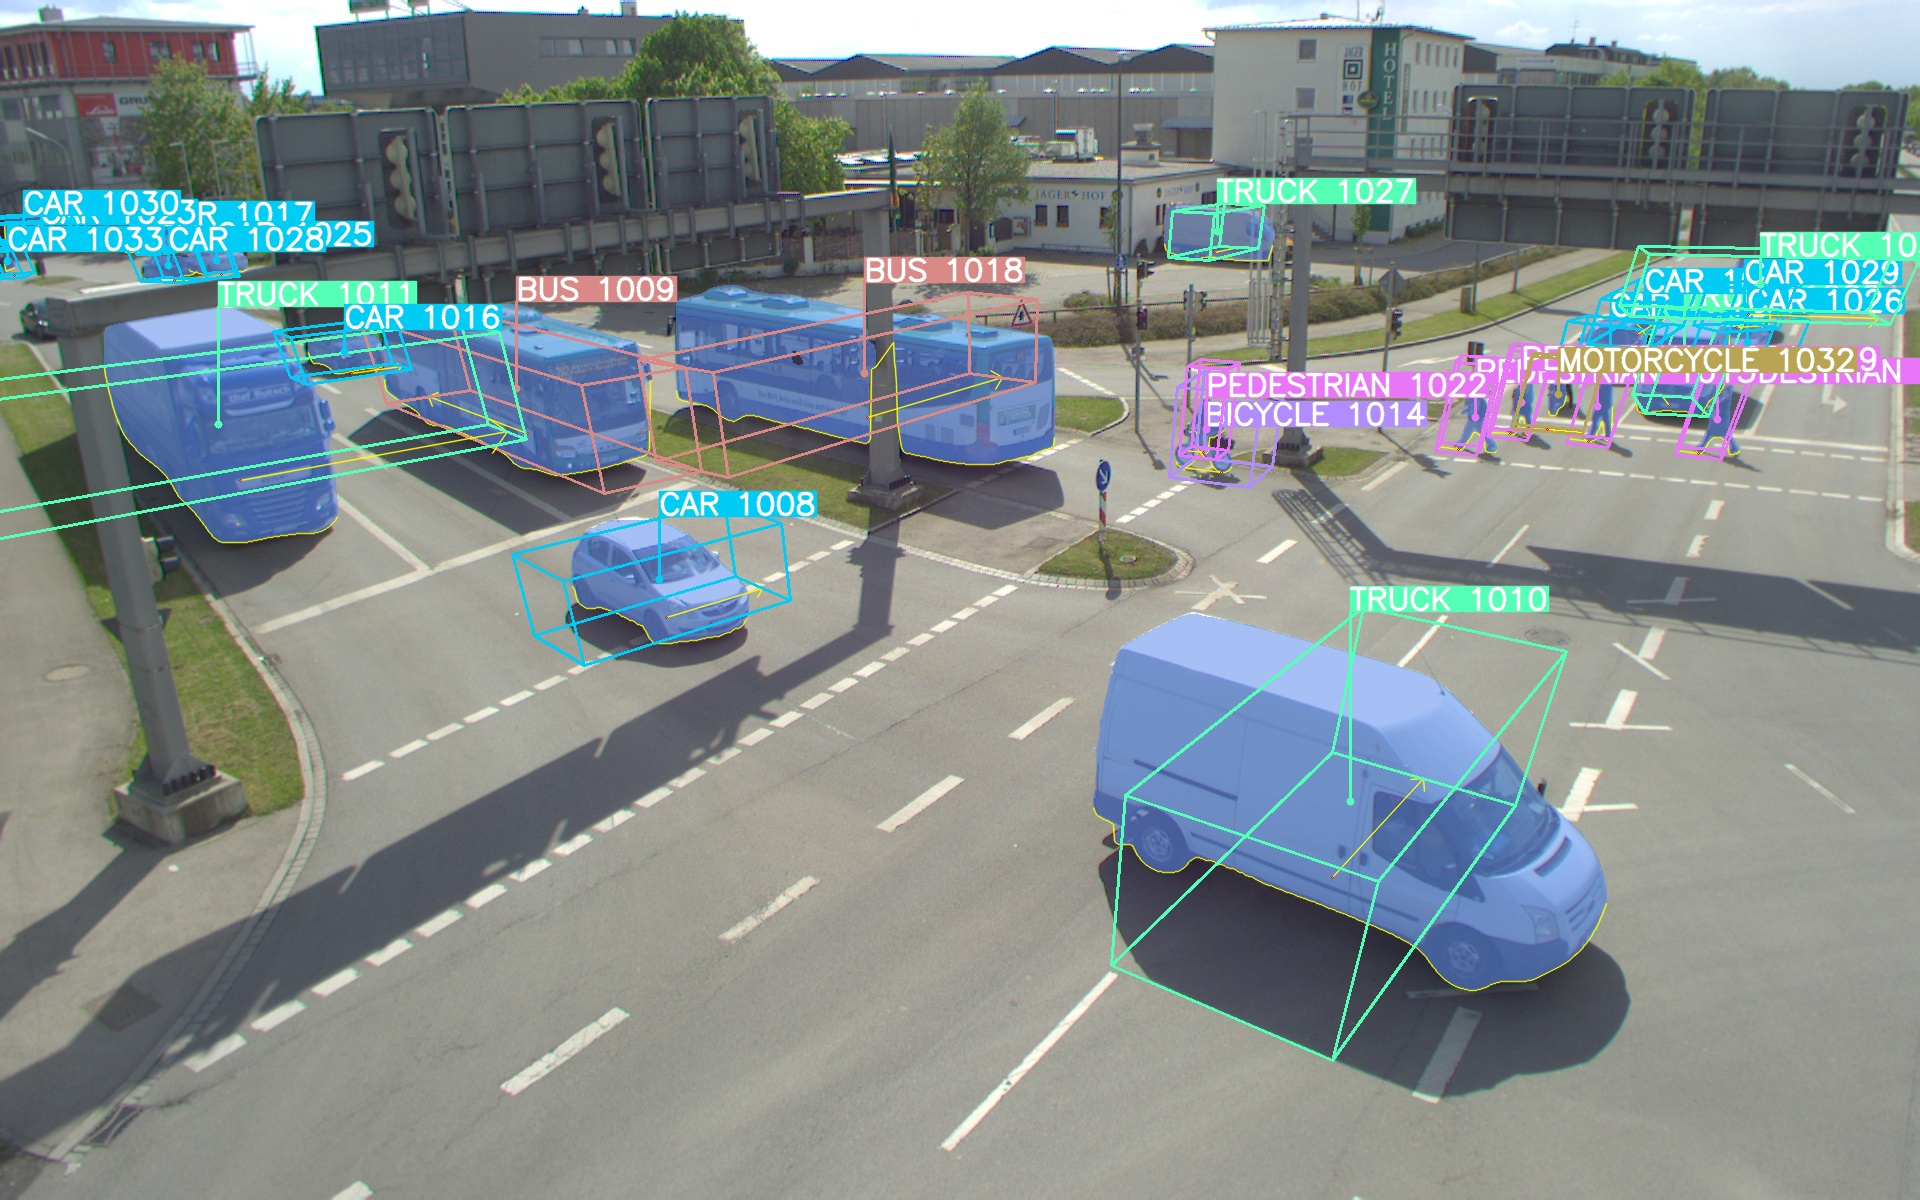
\includegraphics[width=0.45\linewidth]{
        figures/selection/1651673054-274505919-s110-camera-basler-south2-8mm-nomaptrack}
    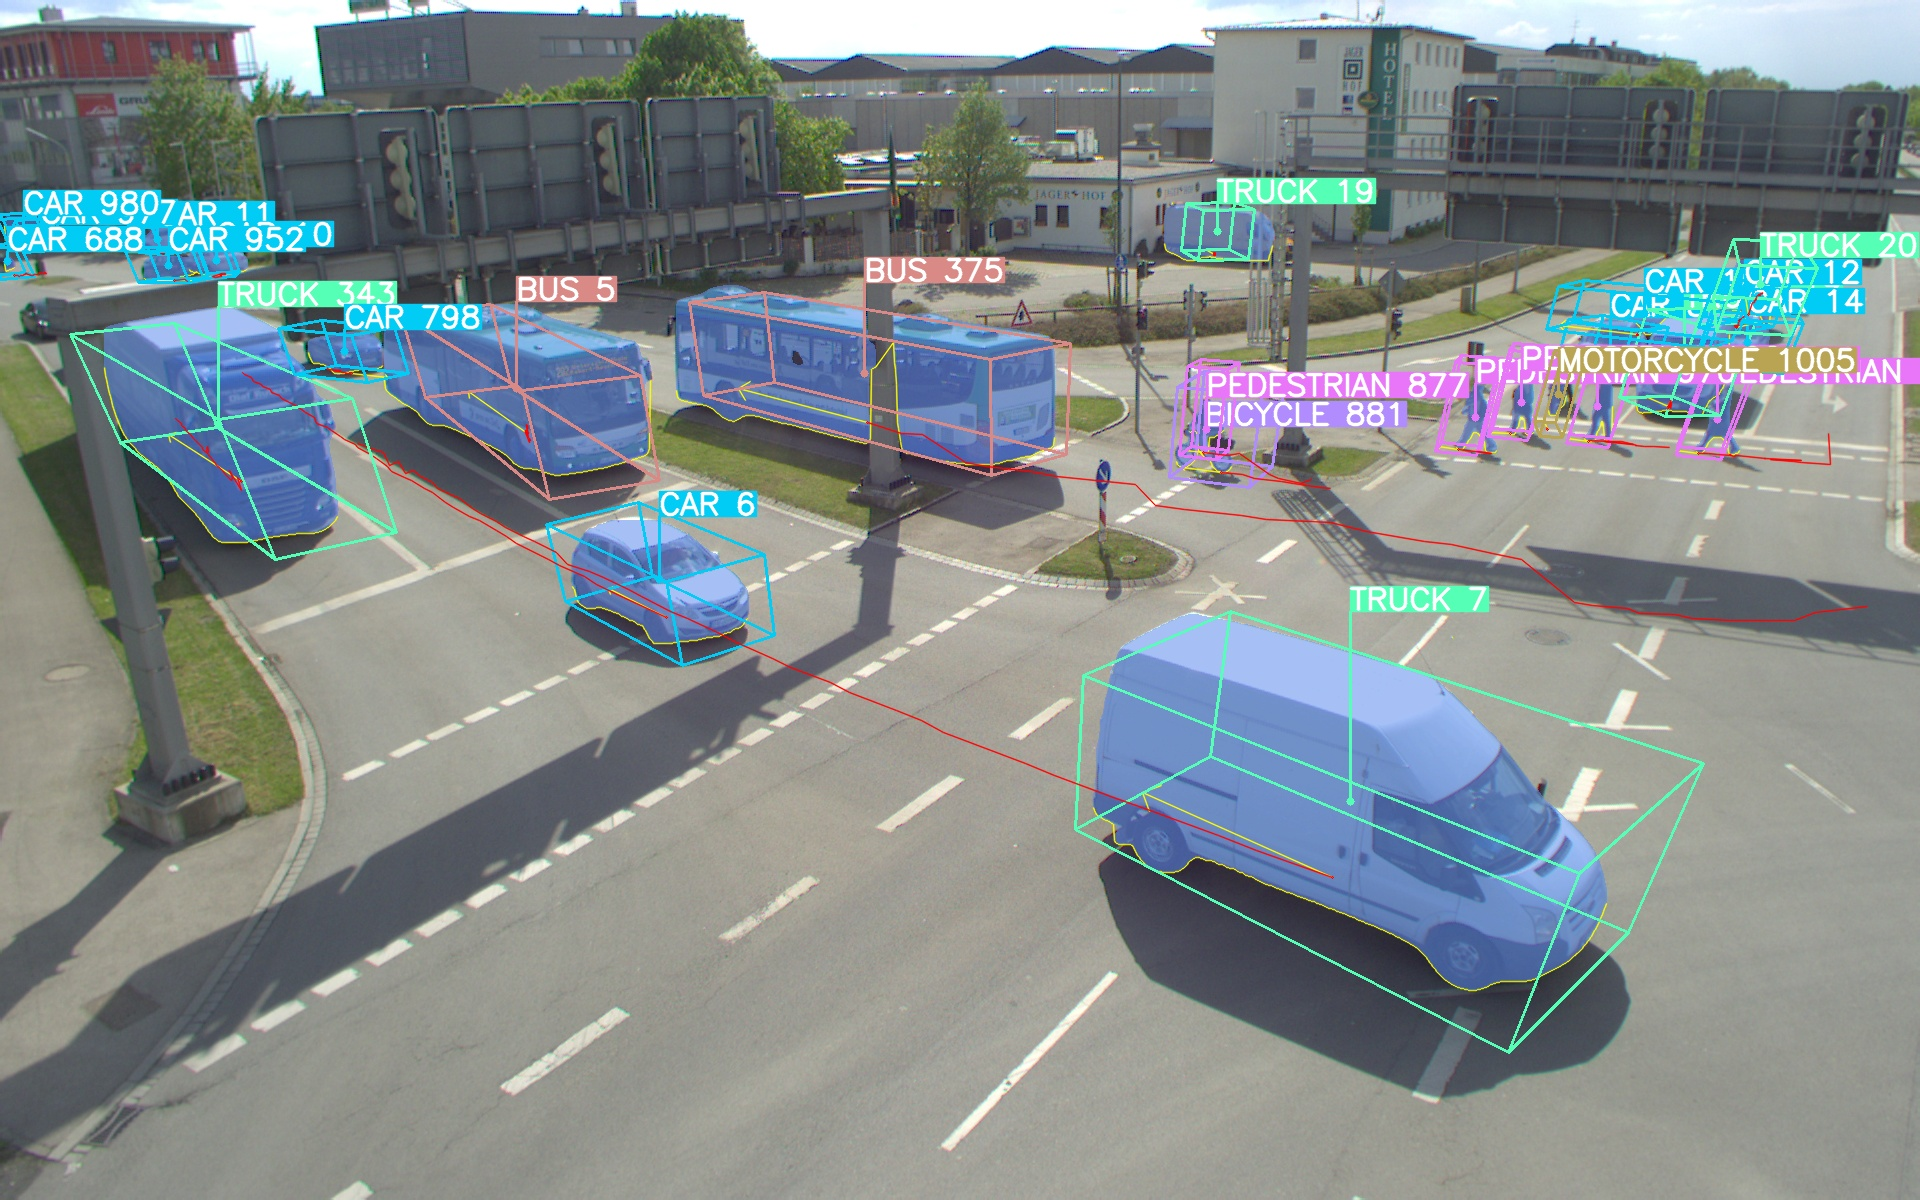
\includegraphics[width=0.45\linewidth]{
        figures/selection/1651673054-274505919-s110-camera-basler-south2-8mm-nomap} \\
    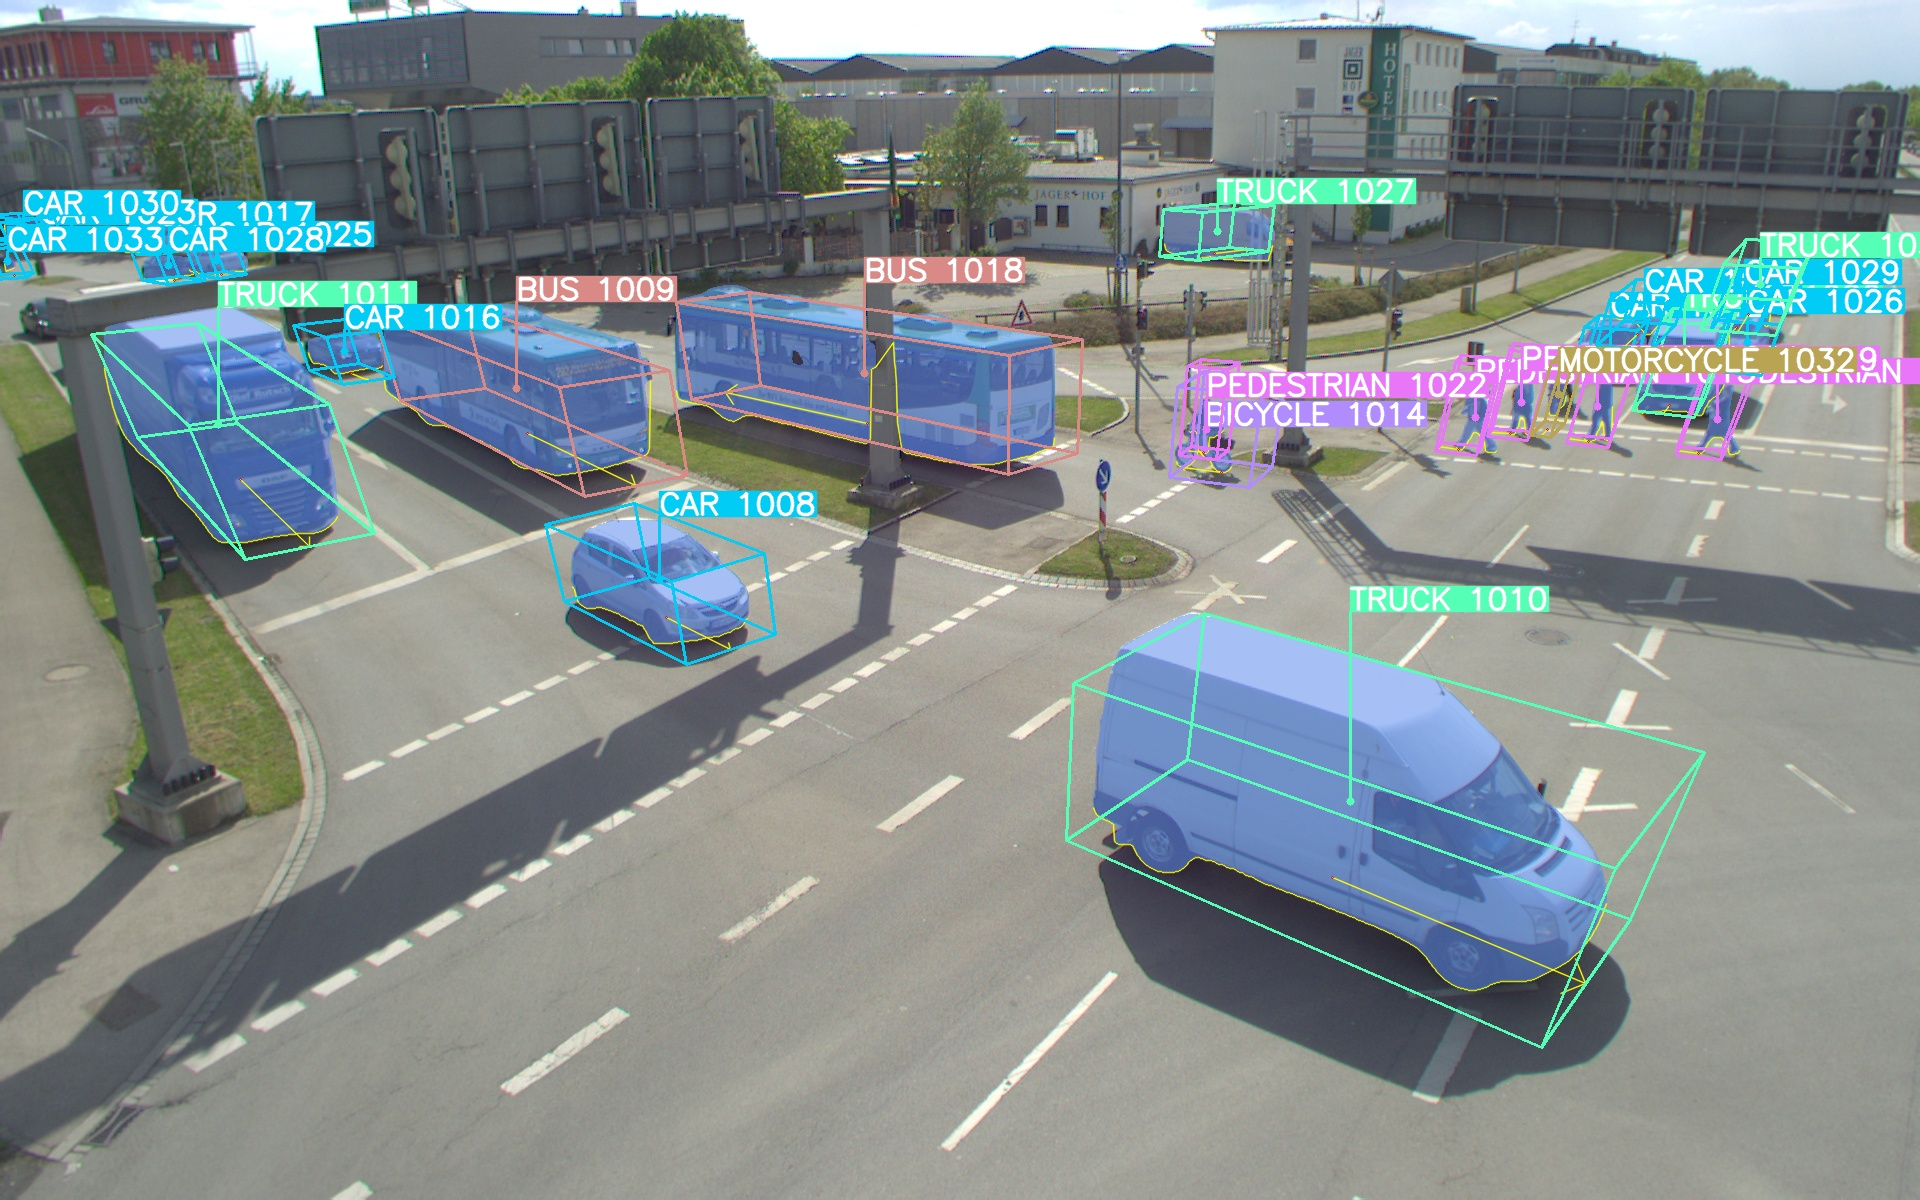
\includegraphics[width=0.45\linewidth]{
        figures/selection/1651673054-274505919-s110-camera-basler-south2-8mm-notrack}
    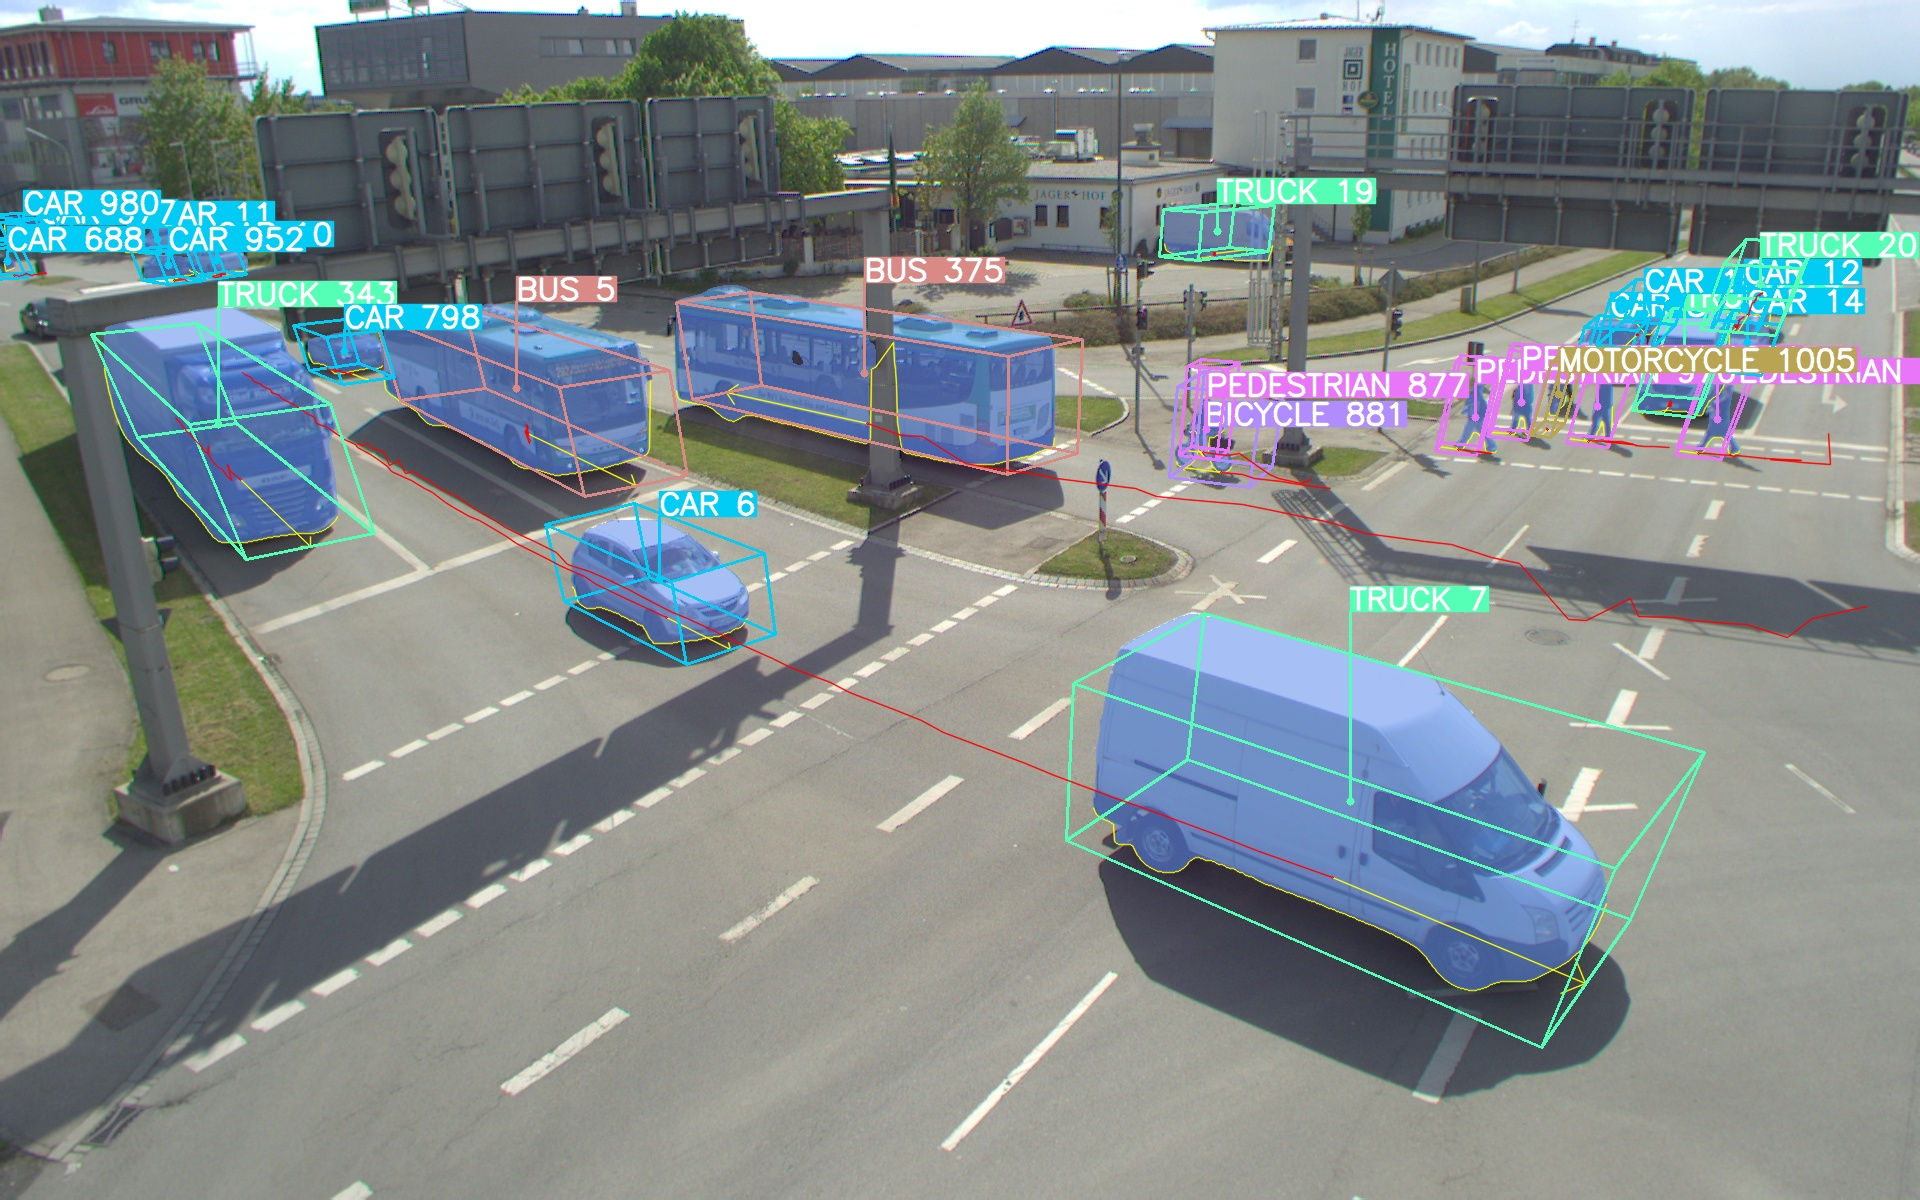
\includegraphics[width=0.45\linewidth]{
        figures/selection/1651673054-274505919-s110-camera-basler-south2-8mm}
    \caption{Comparison of the same frame from our best model ($\left[I^{1920}_\text{Yv7}T_{2D}M_\text{LSF}F_\text{Cont}^\text{Size}\right]$) (bottom-right), vs. the same model except with disabled LSF augmentations (top-left), disabled map augmentation (top-right), or disabled tracking augmentation (bottom-left).}
    \label{fig:qualitative-results-lsf-augments}
\end{figure}

\begin{table*}[h!]
    
        \centering
        \scalebox{0.91}{
        \begin{tabular}{|l|rrrrrr|rrr|}
\hline & \multicolumn{6}{l|}{\textbf{Best w/o LSF Augments} ($\left[I^{1280}_\text{Yv7}T_0M_1F_\text{Size}L_0\right]$)} & \multicolumn{3}{l|}{\textbf{Score}: $35.18\%$ $({\scriptstyle\color{red}-4.98})$} \rule{0pt}{1.4em} \\[0.2em] 

            \hline
            \hline
            \textbf{Class} & \textbf{AOE} & \textbf{ATE} & \textbf{AWE} & \textbf{ALE} & \textbf{AHE} & $\mathbf{IoU}_{3D}$ & \textbf{Precision} & \textbf{Recall} & \textbf{AP}{@}10 \\ 

            \hline
            Vehicle & $43.34\degree$ & $1.17m$ & $0.30m$ & $1.59m$ & $0.53m$ & $35.48\%$ & $58.47\%$ & $50.14\%$ & $57.66\%$ \\ 
Car & $41.03\degree$ & $0.91m$ & $0.25m$ & $0.81m$ & $0.36m$ & $38.15\%$ & $73.62\%$ & $73.21\%$ & $73.11\%$ \\ 
Truck & $55.12\degree$ & $2.94m$ & $0.42m$ & $8.50m$ & $0.82m$ & $18.97\%$ & $32.83\%$ & $33.63\%$ & $32.21\%$ \\ 
Motorcycle & $49.45\degree$ & $0.60m$ & $0.17m$ & $0.20m$ & $0.13m$ & $29.80\%$ & $36.63\%$ & $28.93\%$ & $36.07\%$ \\ 
Bus & $41.89\degree$ & $1.43m$ & $0.47m$ & $2.19m$ & $1.11m$ & $32.66\%$ & $57.03\%$ & $42.12\%$ & $56.17\%$ \\ 
Pedestrian & $26.04\degree$ & $0.26m$ & $0.22m$ & $0.18m$ & $0.06m$ & $28.82\%$ & $13.94\%$ & $7.45\%$ & $13.41\%$ \\ 
Bicycle & $43.64\degree$ & $0.67m$ & $1.18m$ & $0.59m$ & $0.08m$ & $22.82\%$ & $31.29\%$ & $36.10\%$ & $30.99\%$ \\ 

\hline
\textbf{Mean} & $\mathbf{42.93\degree}$ & $\mathbf{1.14m}$ & $\mathbf{0.43m}$ & $\mathbf{2.01m}$ & $\mathbf{0.44m}$ & $\mathbf{29.53\%}$ & $\mathbf{43.40\%}$ & $\mathbf{38.80\%}$ & $\mathbf{42.80\%}$ \\ 
$\Delta$ {Best} & ${\scriptstyle\color{red}+29.13\degree}$ & ${\scriptstyle\color{red}+0.23m}$ & ${\scriptstyle\color{TUMGreen}-0.08m}$ & ${\scriptstyle\color{red}+0.70m}$ & ${\scriptstyle\color{red}+0.05m}$ & ${\scriptstyle\color{red}-0.24\%}$ & ${\scriptstyle\color{TUMGreen}+1.48\%}$ & ${\scriptstyle\color{TUMGreen}+0.94\%}$ & ${\scriptstyle\color{TUMGreen}+1.44\%}$ \\ 

            \hline
            \hline & \multicolumn{6}{l|}{\textbf{Best w/ LSF Tracking-Aug.} ($\left[I^{1920}_\text{Yv7}T_{2D}M_1F_\text{Cont}^\text{Size}L_{\uparrow}\right]$)} & \multicolumn{3}{l|}{\textbf{Score}: $34.95\%$ $({\scriptstyle\color{red}-5.22})$} \rule{0pt}{1.4em} \\[0.2em] 

            \hline
            \hline
            \textbf{Class} & \textbf{AOE} & \textbf{ATE} & \textbf{AWE} & \textbf{ALE} & \textbf{AHE} & $\mathbf{IoU}_{3D}$ & \textbf{Precision} & \textbf{Recall} & \textbf{AP}{@}10 \\ 

            \hline
            Vehicle & $43.18\degree$ & $0.97m$ & $0.37m$ & $1.30m$ & $0.44m$ & $35.48\%$ & $56.70\%$ & $48.11\%$ & $55.88\%$ \\ 
Car & $41.07\degree$ & $0.86m$ & $0.30m$ & $0.88m$ & $0.35m$ & $37.74\%$ & $72.82\%$ & $73.21\%$ & $72.33\%$ \\ 
Truck & $40.53\degree$ & $1.70m$ & $0.65m$ & $2.57m$ & $0.58m$ & $17.95\%$ & $23.91\%$ & $28.91\%$ & $23.23\%$ \\ 
Motorcycle & $57.81\degree$ & $0.76m$ & $0.26m$ & $0.58m$ & $0.14m$ & $27.32\%$ & $35.87\%$ & $31.82\%$ & $35.22\%$ \\ 
Bus & $40.37\degree$ & $1.22m$ & $0.54m$ & $2.94m$ & $1.11m$ & $32.42\%$ & $50.67\%$ & $34.64\%$ & $49.69\%$ \\ 
Pedestrian & $30.97\degree$ & $0.38m$ & $0.28m$ & $0.20m$ & $0.06m$ & $31.71\%$ & $20.86\%$ & $13.62\%$ & $20.47\%$ \\ 
Bicycle & $46.65\degree$ & $0.54m$ & $1.22m$ & $0.70m$ & $0.08m$ & $22.76\%$ & $33.80\%$ & $35.44\%$ & $33.55\%$ \\ 

\hline
\textbf{Mean} & $\mathbf{42.94\degree}$ & $\mathbf{0.92m}$ & $\mathbf{0.52m}$ & $\mathbf{1.31m}$ & $\mathbf{0.40m}$ & $\mathbf{29.34\%}$ & $\mathbf{42.09\%}$ & $\mathbf{37.96\%}$ & $\mathbf{41.48\%}$ \\ 
$\Delta$ {Best} & ${\scriptstyle\color{red}+29.14\degree}$ & ${\scriptstyle\color{red}+0.01m}$ & ${\scriptstyle\color{red}+0.01m}$ & ${\scriptstyle\color{TUMGreen}0.00m}$ & ${\scriptstyle\color{red}+0.01m}$ & ${\scriptstyle\color{red}-0.42\%}$ & ${\scriptstyle\color{TUMGreen}+0.17\%}$ & ${\scriptstyle\color{TUMGreen}+0.11\%}$ & ${\scriptstyle\color{TUMGreen}+0.12\%}$ \\ 

            \hline
            \hline & \multicolumn{6}{l|}{\textbf{Best w/ LSF Map-Aug.} ($\left[I^{1920}_\text{Yv7}T_0M_\text{LSF}F_\text{Cont}^\text{Size}L_{\uparrow}\right]$)} & \multicolumn{3}{l|}{\textbf{Score}: $40.11\%$ $({\scriptstyle\color{red}-0.06})$} \rule{0pt}{1.4em} \\[0.2em] 

            \hline
            \hline
            \textbf{Class} & \textbf{AOE} & \textbf{ATE} & \textbf{AWE} & \textbf{ALE} & \textbf{AHE} & $\mathbf{IoU}_{3D}$ & \textbf{Precision} & \textbf{Recall} & \textbf{AP}{@}10 \\ 

            \hline
            Vehicle & $3.63\degree$ & $0.96m$ & $0.33m$ & $1.30m$ & $0.44m$ & $36.77\%$ & $56.72\%$ & $48.21\%$ & $55.90\%$ \\ 
Car & $3.46\degree$ & $0.85m$ & $0.25m$ & $0.89m$ & $0.35m$ & $39.10\%$ & $72.78\%$ & $73.20\%$ & $72.28\%$ \\ 
Truck & $4.16\degree$ & $1.70m$ & $0.62m$ & $2.51m$ & $0.57m$ & $17.66\%$ & $23.95\%$ & $29.92\%$ & $23.33\%$ \\ 
Motorcycle & $4.06\degree$ & $0.78m$ & $0.31m$ & $0.62m$ & $0.14m$ & $26.89\%$ & $34.46\%$ & $30.49\%$ & $34.02\%$ \\ 
Bus & $6.47\degree$ & $1.19m$ & $0.57m$ & $2.66m$ & $1.13m$ & $35.84\%$ & $51.33\%$ & $35.62\%$ & $50.41\%$ \\ 
Pedestrian & $30.90\degree$ & $0.38m$ & $0.28m$ & $0.20m$ & $0.07m$ & $32.26\%$ & $20.82\%$ & $13.55\%$ & $20.44\%$ \\ 
Bicycle & $40.78\degree$ & $0.56m$ & $1.22m$ & $0.69m$ & $0.08m$ & $21.99\%$ & $33.73\%$ & $35.33\%$ & $33.46\%$ \\ 

\hline
\textbf{Mean} & $\mathbf{13.35\degree}$ & $\mathbf{0.92m}$ & $\mathbf{0.51m}$ & $\mathbf{1.27m}$ & $\mathbf{0.40m}$ & $\mathbf{30.07\%}$ & $\mathbf{41.97\%}$ & $\mathbf{38.05\%}$ & $\mathbf{41.41\%}$ \\ 
$\Delta$ {Best} & ${\scriptstyle\color{TUMGreen}-0.45\degree}$ & ${\scriptstyle\color{red}+0.01m}$ & ${\scriptstyle\color{red}+0.00m}$ & ${\scriptstyle\color{TUMGreen}-0.04m}$ & ${\scriptstyle\color{red}+0.01m}$ & ${\scriptstyle\color{TUMGreen}+0.31\%}$ & ${\scriptstyle\color{TUMGreen}+0.05\%}$ & ${\scriptstyle\color{TUMGreen}+0.19\%}$ & ${\scriptstyle\color{TUMGreen}+0.04\%}$ \\ 

            \hline
            
        \end{tabular}
        }
    \caption{Ablation study for the best model $\left[I^{1920}_\text{Yv7}T_{2D}M_\text{LSF}F_\text{Cont}^\text{Size}\right]$, when none or just one of the Screen-Space-Tracking or HD-Map-Lookup Augmentations for the L-Shape-Fitting (LSF) algorithm is used.}
    \label{tbl:lsf-results}
\end{table*}

\subsection{Impact of HD Map Augmentation}
\label{subsec:impactmap}

Table~\ref{tbl:lsf-results} provides ablated performance metrics for the best-performing model.
First off, when no augmentations are used, the same model's performance drops by $9.67$\%.
When only the HD map augmentation is used, the model reaches a Score of $40.11$\%, which is only $0.06$\% lower than that of the best model, which uses both LSF Augments.
The mean Average Orientation Error (AOE) is significantly reduced to $3.63~\degree$, which is still below the best's performance by $0.16~\degree$.
Overall, the HD-map-input LSF augmentation demonstrates a very positive impact on the detector's performance, but it alone does not beat the top model.

\subsection{Impact of Screen-Space Tracking Augmentation}
\label{subsec:impactlsf}

When the best-performing uses only the Screen-Space Tracking LSF augmentation it reaches a Score of $38.02\%$, which is $7.99\%$ lower than the best model.
Compared to the best un-augmented model, the mean AOE is slightly improved to $48.41\degree$.
Overall, the sole screen-space-tracking LSF augmentation shows some improvements towards the un-augmented model but does not reach the best's performance.
We can conclude that Tracking alone is insufficient as a bias for vehicle orientation estimation.
However, the final best model still uses this augmentation in conjunction with the HD map, and thereby manages to reach the highest score.

% ----------------------------------------------------

\section{Significance of 3D Tracking}
\label{sec:impacttracking}

In this section, we discuss the evaluation results for the 3D SORT tracking technique, as described in Section~\ref{sec:trackthreed} and presented in Table~\ref{tbl:track-3d-results}.

The results demonstrate that the 3D SORT tracking approach led to a decrease in overall performance compared to the best configuration without 3D tracking.
Although there were some minor improvements in certain aspects, such as a decrease in Absolute Translation Error (ATE) by $0.04~m$, the overall score dropped by $1.07\%$, with reductions in Precision, Recall, and mAP.
In conclusion, the 3D SORT tracking technique, as implemented in this study, did not improve the overall performance.
As mentioned in Section~\ref{sec:trackthreed}, a more capable Kalman Filter that takes vehicle heading into account is needed for better performance in 3D tracking.

\begin{table*}[h!]
    
        \centering
        \scalebox{0.91}{
        \begin{tabular}{|l|rrrrrr|rrr|}
\hline & \multicolumn{6}{l|}{\textbf{Best w/ 3D Tracking} ($\left[I^{1920}_\text{Yv7}T_{3D}M_\text{LSF}F_\text{Cont}^\text{Size}L_{\uparrow}\right]$)} & \multicolumn{3}{l|}{\textbf{Score}: $39.22\%$ $({\scriptstyle\color{red}-1.07\%})$} \rule{0pt}{1.4em} \\[0.2em] 

            \hline
            \hline
            \textbf{Class} & \textbf{AOE} & \textbf{ATE} & \textbf{AWE} & \textbf{ALE} & \textbf{AHE} & $\mathbf{IoU}_{3D}$ & \textbf{Precision} & \textbf{Recall} & \textbf{AP}{@}10 \\ 

            \hline
            Car & $3.46\degree$ & $0.85m$ & $0.29m$ & $1.19m$ & $0.35m$ & $36.12\%$ & $71.35\%$ & $72.39\%$ & $70.85\%$ \\ 
Truck & $4.14\degree$ & $1.47m$ & $0.74m$ & $2.03m$ & $0.68m$ & $18.44\%$ & $17.87\%$ & $22.40\%$ & $17.30\%$ \\ 
Motorcycle & $4.04\degree$ & $0.78m$ & $0.35m$ & $0.62m$ & $0.14m$ & $24.26\%$ & $33.61\%$ & $30.23\%$ & $33.28\%$ \\ 
Bus & $7.29\degree$ & $1.14m$ & $0.51m$ & $1.99m$ & $1.23m$ & $36.89\%$ & $48.12\%$ & $31.80\%$ & $47.09\%$ \\ 
Pedestrian & \textemdash & $0.38m$ & $0.28m$ & $0.20m$ & $0.06m$ & $32.06\%$ & $20.93\%$ & $13.70\%$ & $20.54\%$ \\ 
Bicycle & \textemdash & $0.55m$ & $1.22m$ & $0.69m$ & $0.08m$ & $22.22\%$ & $33.77\%$ & $35.44\%$ & $33.52\%$ \\ 

\hline
\textbf{Mean} & $\mathbf{4.73\degree}$ & $\mathbf{0.86m}$ & $\mathbf{0.56m}$ & $\mathbf{1.12m}$ & $\mathbf{0.42m}$ & $\mathbf{28.33\%}$ & $\mathbf{37.61\%}$ & $\mathbf{34.33\%}$ & $\mathbf{37.10\%}$ \\ 
$\Delta$ {Best} & ${\scriptstyle\color{TUMGreen}-0.64\degree}$ & ${\scriptstyle\color{TUMGreen}-0.04m}$ & ${\scriptstyle\color{red}+0.02m}$ & ${\scriptstyle\color{TUMGreen}-0.19m}$ & ${\scriptstyle\color{red}+0.04m}$ & ${\scriptstyle\color{red}-0.26\%}$ & ${\scriptstyle\color{red}-1.85\%}$ & ${\scriptstyle\color{red}-1.81\%}$ & ${\scriptstyle\color{red}-1.85\%}$ \\ 

            \hline
            
        \end{tabular}
        }
    \caption{Best result for model which uses 3D Tracking, compared with the best model.}
    \label{tbl:track-3d-results}
\end{table*}

\begin{table*}[h!]
    
        \centering
        \scalebox{0.91}{
        \begin{tabular}{|l|rrrrrr|rrr|}
\hline & \multicolumn{6}{l|}{\textbf{Average Results Using Original Labels}} & \multicolumn{3}{l|}{\textbf{PDS}: $28.13\%$} \rule{0pt}{1.4em} \\[0.2em] 

            \hline
            \hline
            \textbf{Class} & \textbf{AOE} & \textbf{ATE} & \textbf{AWE} & \textbf{ALE} & \textbf{AHE} & $\mathbf{IoU}_{3D}$ & \textbf{Precision} & \textbf{Recall} & \textbf{AP}{@}10 \\ 

            \hline
            Car & $32.47\degree$ & $0.92\nobreak\hspace{{.16667em plus .08333em}}m$ & $0.39\nobreak\hspace{{.16667em plus .08333em}}m$ & $1.09\nobreak\hspace{{.16667em plus .08333em}}m$ & $0.45\nobreak\hspace{{.16667em plus .08333em}}m$ & $31.27\%$ & $60.24\%$ & $58.87\%$ & $59.61\%$ \\ 
Truck & $29.86\degree$ & $2.08\nobreak\hspace{{.16667em plus .08333em}}m$ & $0.78\nobreak\hspace{{.16667em plus .08333em}}m$ & $4.34\nobreak\hspace{{.16667em plus .08333em}}m$ & $0.82\nobreak\hspace{{.16667em plus .08333em}}m$ & $18.59\%$ & $12.91\%$ & $13.27\%$ & $12.26\%$ \\ 
Motorcycle & $34.00\degree$ & $0.63\nobreak\hspace{{.16667em plus .08333em}}m$ & $0.35\nobreak\hspace{{.16667em plus .08333em}}m$ & $0.63\nobreak\hspace{{.16667em plus .08333em}}m$ & $0.12\nobreak\hspace{{.16667em plus .08333em}}m$ & $23.75\%$ & $34.79\%$ & $27.87\%$ & $34.35\%$ \\ 
Bus & $29.55\degree$ & $1.48\nobreak\hspace{{.16667em plus .08333em}}m$ & $0.93\nobreak\hspace{{.16667em plus .08333em}}m$ & $2.99\nobreak\hspace{{.16667em plus .08333em}}m$ & $1.21\nobreak\hspace{{.16667em plus .08333em}}m$ & $27.65\%$ & $38.20\%$ & $25.15\%$ & $37.15\%$ \\ 
Pedestrian & \textemdash & $0.34\nobreak\hspace{{.16667em plus .08333em}}m$ & $0.24\nobreak\hspace{{.16667em plus .08333em}}m$ & $0.20\nobreak\hspace{{.16667em plus .08333em}}m$ & $0.07\nobreak\hspace{{.16667em plus .08333em}}m$ & $26.39\%$ & $10.52\%$ & $5.55\%$ & $10.05\%$ \\ 
Bicycle & \textemdash & $0.53\nobreak\hspace{{.16667em plus .08333em}}m$ & $1.02\nobreak\hspace{{.16667em plus .08333em}}m$ & $0.55\nobreak\hspace{{.16667em plus .08333em}}m$ & $0.09\nobreak\hspace{{.16667em plus .08333em}}m$ & $23.87\%$ & $19.50\%$ & $17.97\%$ & $19.09\%$ \\ 

\hline
\textbf{Mean} & $\mathbf{31.47\degree}$ & $\mathbf{1.00\nobreak\hspace{{.16667em plus .08333em}}m}$ & $\mathbf{0.62\nobreak\hspace{{.16667em plus .08333em}}m}$ & $\mathbf{1.63\nobreak\hspace{{.16667em plus .08333em}}m}$ & $\mathbf{0.46\nobreak\hspace{{.16667em plus .08333em}}m}$ & $\mathbf{25.25\%}$ & $\mathbf{29.36\%}$ & $\mathbf{24.78\%}$ & $\mathbf{28.75\%}$ \\ 

            \hline
            \hline & \multicolumn{6}{l|}{\textbf{Average Results Using Time-Shifted Labels}} & \multicolumn{3}{l|}{\textbf{PDS}: $28.16\%$ $({\scriptstyle\color{TUMGreen}+0.02\%})$} \rule{0pt}{1.4em} \\[0.2em] 

            \hline
            \hline
            \textbf{Class} & \textbf{AOE} & \textbf{ATE} & \textbf{AWE} & \textbf{ALE} & \textbf{AHE} & $\mathbf{IoU}_{3D}$ & \textbf{Precision} & \textbf{Recall} & \textbf{AP}{@}10 \\ 

            \hline
            Car & $32.44\degree$ & $0.90\nobreak\hspace{{.16667em plus .08333em}}m$ & $0.39\nobreak\hspace{{.16667em plus .08333em}}m$ & $1.08\nobreak\hspace{{.16667em plus .08333em}}m$ & $0.45\nobreak\hspace{{.16667em plus .08333em}}m$ & $31.50\%$ & $61.02\%$ & $59.71\%$ & $60.38\%$ \\ 
Truck & $30.03\degree$ & $2.10\nobreak\hspace{{.16667em plus .08333em}}m$ & $0.78\nobreak\hspace{{.16667em plus .08333em}}m$ & $4.35\nobreak\hspace{{.16667em plus .08333em}}m$ & $0.83\nobreak\hspace{{.16667em plus .08333em}}m$ & $17.98\%$ & $12.64\%$ & $13.29\%$ & $12.09\%$ \\ 
Motorcycle & $33.93\degree$ & $0.62\nobreak\hspace{{.16667em plus .08333em}}m$ & $0.35\nobreak\hspace{{.16667em plus .08333em}}m$ & $0.65\nobreak\hspace{{.16667em plus .08333em}}m$ & $0.15\nobreak\hspace{{.16667em plus .08333em}}m$ & $23.23\%$ & $35.59\%$ & $28.06\%$ & $35.15\%$ \\ 
Bus & $29.60\degree$ & $1.41\nobreak\hspace{{.16667em plus .08333em}}m$ & $0.98\nobreak\hspace{{.16667em plus .08333em}}m$ & $3.01\nobreak\hspace{{.16667em plus .08333em}}m$ & $1.25\nobreak\hspace{{.16667em plus .08333em}}m$ & $27.62\%$ & $38.14\%$ & $25.14\%$ & $37.09\%$ \\ 
Pedestrian & \textemdash & $0.33\nobreak\hspace{{.16667em plus .08333em}}m$ & $0.24\nobreak\hspace{{.16667em plus .08333em}}m$ & $0.17\nobreak\hspace{{.16667em plus .08333em}}m$ & $0.06\nobreak\hspace{{.16667em plus .08333em}}m$ & $26.91\%$ & $10.45\%$ & $5.58\%$ & $9.99\%$ \\ 
Bicycle & \textemdash & $0.47\nobreak\hspace{{.16667em plus .08333em}}m$ & $1.05\nobreak\hspace{{.16667em plus .08333em}}m$ & $0.63\nobreak\hspace{{.16667em plus .08333em}}m$ & $0.09\nobreak\hspace{{.16667em plus .08333em}}m$ & $23.21\%$ & $19.03\%$ & $17.37\%$ & $18.62\%$ \\ 

\hline
\textbf{Mean} & $\mathbf{31.50\degree}$ & $\mathbf{0.97\nobreak\hspace{{.16667em plus .08333em}}m}$ & $\mathbf{0.63\nobreak\hspace{{.16667em plus .08333em}}m}$ & $\mathbf{1.65\nobreak\hspace{{.16667em plus .08333em}}m}$ & $\mathbf{0.47\nobreak\hspace{{.16667em plus .08333em}}m}$ & $\mathbf{25.08\%}$ & $\mathbf{29.48\%}$ & $\mathbf{24.86\%}$ & $\mathbf{28.89\%}$ \\ 
$\Delta$ {Previous} & ${\scriptstyle\color{red}+0.03\degree}$ & ${\scriptstyle\color{TUMGreen}-0.02\nobreak\hspace{{.16667em plus .08333em}}m}$ & ${\scriptstyle\color{red}+0.01\nobreak\hspace{{.16667em plus .08333em}}m}$ & ${\scriptstyle\color{red}+0.01\nobreak\hspace{{.16667em plus .08333em}}m}$ & ${\scriptstyle\color{red}+0.01\nobreak\hspace{{.16667em plus .08333em}}m}$ & ${\scriptstyle\color{red}-0.18\%}$ & ${\scriptstyle\color{TUMGreen}+0.12\%}$ & ${\scriptstyle\color{TUMGreen}+0.08\%}$ & ${\scriptstyle\color{TUMGreen}+0.14\%}$ \\ 

            \hline
            
        \end{tabular}
        }
    \caption{Average results for evaluations with time-shifted labels compared to the original unsynchronized LiDAR labels.}
    \label{tbl:label-shift-results}
\end{table*}

\section{Implications of LiDAR Label Shifting}
\label{sec:impactlidar}

In this section, we discuss the evaluation results of the LiDAR label shifting technique, as described in Section~\ref{sec:quant} and presented in Table~\ref{tbl:label-shift-results}.

The results indicate that using time-shifted LiDAR labels ($L_{\uparrow}$) led to a minor improvement in the overall performance compared to using original LiDAR labels ($L_0$).
The overall score increased by $0.02\%$, with small improvements in Precision, Recall, and mAP.

Overall, the LiDAR label shifting technique using SORT for estimating spatial velocity and correcting label positions based on the known synchronization error time delta led to a slight improvement in overall performance.
Although the improvements are minor, they demonstrate that accounting for sensor delay between camera and LiDAR sensor frames can help reduce the inherent offset in the LiDAR labels and improve evaluation accuracy.

% ----------------------------------------------------

\section{Challenges of Night-time Conditions}
\label{sec:weather}

As discussed in the qualitative analysis, the detection performance of a system that relies on an RGB camera operating within the human visible light spectrum is expected to be worse at night due to the reduced visibility.
The results in Table~\ref{tbl:nighttime-results} quantitatively confirm this expectation, showing that both \textit{Yolact-Edge} and \textit{Yolov7} models exhibit degraded performance under night-time conditions.

\begin{table*}[h!]
    
        \centering
        \scalebox{0.91}{
        \begin{tabular}{|l|rrrrrr|rrr|}
\hline & \multicolumn{6}{l|}{\textbf{Average Night-Time Results Using Yolact-Edge}} & \multicolumn{3}{l|}{\textbf{Score}: $21.13\%$} \rule{0pt}{1.4em} \\[0.2em] 

            \hline
            \hline
            \textbf{Class} & \textbf{AOE} & \textbf{ATE} & \textbf{AWE} & \textbf{ALE} & \textbf{AHE} & $\mathbf{IoU}_{3D}$ & \textbf{Precision} & \textbf{Recall} & \textbf{AP}{@}10 \\ 

            \hline
            Car & $40.07\degree$ & $0.94m$ & $0.32m$ & $1.29m$ & $0.54m$ & $31.57\%$ & $39.74\%$ & $26.44\%$ & $38.55\%$ \\ 
Truck & $22.71\degree$ & $2.33m$ & $0.38m$ & $3.93m$ & $1.31m$ & $18.70\%$ & $0.65\%$ & $0.19\%$ & $0.44\%$ \\ 
Motorcycle & \textemdash & \textemdash & \textemdash & \textemdash & \textemdash & \textemdash & \textemdash & \textemdash & \textemdash \\ 
Bus & $30.01\degree$ & $1.22m$ & $0.83m$ & $2.16m$ & $1.48m$ & $29.71\%$ & $31.99\%$ & $18.15\%$ & $30.76\%$ \\ 
Pedestrian & \textemdash & \textemdash & \textemdash & \textemdash & \textemdash & \textemdash & \textemdash & \textemdash & \textemdash \\ 
Bicycle & \textemdash & \textemdash & \textemdash & \textemdash & \textemdash & \textemdash & \textemdash & \textemdash & \textemdash \\ 

\hline
\textbf{Mean} & $\mathbf{30.93\degree}$ & $\mathbf{1.50m}$ & $\mathbf{0.51m}$ & $\mathbf{2.46m}$ & $\mathbf{1.11m}$ & $\mathbf{26.66\%}$ & $\mathbf{24.12\%}$ & $\mathbf{14.93\%}$ & $\mathbf{23.25\%}$ \\ 

            \hline
            \hline & \multicolumn{6}{l|}{\textbf{Average Night-Time Results Using Yolov7}} & \multicolumn{3}{l|}{\textbf{Score}: $24.99\%$ $({\scriptstyle\color{TUMGreen}+3.86\%})$} \rule{0pt}{1.4em} \\[0.2em] 

            \hline
            \hline
            \textbf{Class} & \textbf{AOE} & \textbf{ATE} & \textbf{AWE} & \textbf{ALE} & \textbf{AHE} & $\mathbf{IoU}_{3D}$ & \textbf{Precision} & \textbf{Recall} & \textbf{AP}{@}10 \\ 

            \hline
            Car & $34.38\degree$ & $0.96m$ & $0.38m$ & $1.20m$ & $0.48m$ & $29.62\%$ & $45.17\%$ & $37.03\%$ & $44.20\%$ \\ 
Truck & $24.64\degree$ & $1.46m$ & $0.41m$ & $2.69m$ & $0.58m$ & $11.80\%$ & $3.82\%$ & $2.25\%$ & $3.34\%$ \\ 
Motorcycle & \textemdash & \textemdash & \textemdash & \textemdash & \textemdash & \textemdash & \textemdash & \textemdash & \textemdash \\ 
Bus & $26.71\degree$ & $1.28m$ & $0.92m$ & $2.54m$ & $1.07m$ & $28.34\%$ & $30.36\%$ & $15.65\%$ & $29.16\%$ \\ 
Pedestrian & \textemdash & \textemdash & \textemdash & \textemdash & \textemdash & \textemdash & \textemdash & \textemdash & \textemdash \\ 
Bicycle & \textemdash & \textemdash & \textemdash & \textemdash & \textemdash & \textemdash & \textemdash & \textemdash & \textemdash \\ 

\hline
\textbf{Mean} & $\mathbf{28.58\degree}$ & $\mathbf{1.23m}$ & $\mathbf{0.57m}$ & $\mathbf{2.14m}$ & $\mathbf{0.71m}$ & $\mathbf{23.25\%}$ & $\mathbf{26.45\%}$ & $\mathbf{18.31\%}$ & $\mathbf{25.57\%}$ \\ 
$\Delta$ {Previous} & ${\scriptstyle\color{TUMGreen}-2.35\degree}$ & ${\scriptstyle\color{TUMGreen}-0.27m}$ & ${\scriptstyle\color{red}+0.06m}$ & ${\scriptstyle\color{TUMGreen}-0.31m}$ & ${\scriptstyle\color{TUMGreen}-0.40m}$ & ${\scriptstyle\color{red}-3.41\%}$ & ${\scriptstyle\color{TUMGreen}+2.33\%}$ & ${\scriptstyle\color{TUMGreen}+3.38\%}$ & ${\scriptstyle\color{TUMGreen}+2.32\%}$ \\ 

            \hline
            
        \end{tabular}
        }
    \caption{Average results for evaluations on the night-time scene of the A9 dataset with \textit{Yolact-Edge} and \textit{Yolov7} models.}
    \label{tbl:nighttime-results}
\end{table*}

When comparing the night-time results, it is evident that the \textit{Yolov7} model outperforms the Yolact-Edge model in most of the considered evaluation metrics.
The overall score for the Yolov7 model is $24.99\%$, which is an improvement of $3.86\%$ compared to the Yolact-Edge model.
This improvement can be primarily attributed to the higher precision and recall rates, as well as a reduced average translation error (ATE) and average length error (ALE).

Despite the degraded performance at night, the \textit{Yolov7} instance segmentation model still demonstrates a reasonable level of detection accuracy for certain object classes, such as cars and buses.
However, for some classes like trucks, the average precision drops significantly, indicating a higher rate of false positives and false negatives.

It is also important to note that the performance for certain object classes like motorcycles, pedestrians, and bicycles is not reported in the night-time evaluation.
This is due to a lack of evaluation samples for these classes in the night-time dataset scene.

In summary, the quantitative evaluation confirms the expected reduction in detection performance under night-time conditions.
While the \textit{Yolov7} model demonstrates better performance compared to the \textit{Yolact-Edge} model, further research and development are necessary to improve the overall performance of instance segmentation models in low-light and night-time environments.

\section{Perspective-Dependent Detector Performance}
\label{sec:perspective}

The detection performance can be significantly influenced by the camera perspective.
In this work, we analyze the impact of two different camera perspectives from the A9 test field: \texttt{S110-S1} and \texttt{S110-S2}.
The \texttt{S110-S1} camera is focused downwards onto the intersection, whereas the \texttt{S110-S2} camera has a longer detection range and is angled towards the horizon.
In this section, we provide a quantitative comparison of the best-performing models for each perspective, focusing on the vehicle super-category, which emphasizes the shape detection performance rather than the object classification aspect.

Table~\ref{tbl:perspective-results} shows the quantitative results for the best-performing vehicle-only models for each camera perspective.

\begin{table*}[htb]
    
        \centering
        \scalebox{0.91}{
        \begin{tabular}{|l|rrrrrr|rrr|}
\hline & \multicolumn{6}{l|}{\textbf{Best for S110-S1 Perspective:} $\left[I^{550}_\text{YOL}T_0M_\text{LSF}F_\text{Cont}^\text{Size}L_0\right]$} & \multicolumn{3}{l|}{\textbf{PDS}: $55.60\%$ $({\scriptstyle\color{TUMGreen}+5.53\%})$} \rule{0pt}{1.4em} \\[0.2em] 

            \hline
            \hline
            \textbf{Class} & \textbf{AOE} & \textbf{ATE} & \textbf{AWE} & \textbf{ALE} & \textbf{AHE} & $\mathbf{IoU}_{3D}$ & \textbf{Precision} & \textbf{Recall} & \textbf{AP}{@}10 \\ 

            \hline
            Vehicle & $3.90\degree$ & $1.04\nobreak\hspace{{.16667em plus .08333em}}m$ & $0.31\nobreak\hspace{{.16667em plus .08333em}}m$ & $1.34\nobreak\hspace{{.16667em plus .08333em}}m$ & $0.34\nobreak\hspace{{.16667em plus .08333em}}m$ & $39.90\%$ & $66.05\%$ & $55.82\%$ & $65.54\%$ \\ 
$\Delta$ {Best} & ${\scriptstyle\color{red}+0.43\degree}$ & ${\scriptstyle\color{red}+0.08\nobreak\hspace{{.16667em plus .08333em}}m}$ & ${\scriptstyle\color{TUMGreen}-0.02\nobreak\hspace{{.16667em plus .08333em}}m}$ & ${\scriptstyle\color{red}+0.03\nobreak\hspace{{.16667em plus .08333em}}m}$ & ${\scriptstyle\color{TUMGreen}-0.10\nobreak\hspace{{.16667em plus .08333em}}m}$ & ${\scriptstyle\color{TUMGreen}+3.11\%}$ & ${\scriptstyle\color{TUMGreen}+9.33\%}$ & ${\scriptstyle\color{TUMGreen}+7.64\%}$ & ${\scriptstyle\color{TUMGreen}+9.64\%}$ \\ 

            \hline
            \hline & \multicolumn{6}{l|}{\textbf{Best for S110-S2 Perspective:} $\left[I^{640}_\text{Yv7}T^{2D}_{3D}M_\text{LSF}F_\text{Size}L_0\right]$} & \multicolumn{3}{l|}{\textbf{PDS}: $50.90\%$ $({\scriptstyle\color{TUMGreen}+0.83\%})$} \rule{0pt}{1.4em} \\[0.2em] 

            \hline
            \hline
            \textbf{Class} & \textbf{AOE} & \textbf{ATE} & \textbf{AWE} & \textbf{ALE} & \textbf{AHE} & $\mathbf{IoU}_{3D}$ & \textbf{Precision} & \textbf{Recall} & \textbf{AP}{@}10 \\ 

            \hline
            Vehicle & $3.43\degree$ & $0.93\nobreak\hspace{{.16667em plus .08333em}}m$ & $0.29\nobreak\hspace{{.16667em plus .08333em}}m$ & $1.49\nobreak\hspace{{.16667em plus .08333em}}m$ & $0.66\nobreak\hspace{{.16667em plus .08333em}}m$ & $35.52\%$ & $61.39\%$ & $51.79\%$ & $60.69\%$ \\ 
$\Delta$ {Best} & ${\scriptstyle\color{TUMGreen}-0.04\degree}$ & ${\scriptstyle\color{TUMGreen}-0.02\nobreak\hspace{{.16667em plus .08333em}}m}$ & ${\scriptstyle\color{TUMGreen}-0.04\nobreak\hspace{{.16667em plus .08333em}}m}$ & ${\scriptstyle\color{red}+0.19\nobreak\hspace{{.16667em plus .08333em}}m}$ & ${\scriptstyle\color{red}+0.22\nobreak\hspace{{.16667em plus .08333em}}m}$ & ${\scriptstyle\color{red}-1.27\%}$ & ${\scriptstyle\color{TUMGreen}+4.67\%}$ & ${\scriptstyle\color{TUMGreen}+3.62\%}$ & ${\scriptstyle\color{TUMGreen}+4.79\%}$ \\ 

            \hline
            
        \end{tabular}
        }
    \caption{Quantitative results for the best-performing vehicle-only models for each camera perspective.}
    \label{tbl:perspective-results}
\end{table*}

For the \texttt{S110-S1} perspective, the best vehicle-only model achieves a score of $55.60\%$, which is an improvement of $5.53\%$ over the best model for both perspectives.
Most interestingly, this best model uses \textit{Yolact-Edge}.
But as Table~\ref{tbl:perspective-results-switched} shows, this model does not transfer its performance to \texttt{S110-S2}.

For the \texttt{S110-S2} perspective, the best vehicle-only model obtains a score of $50.90\%$, with a performance improvement of $0.83\%$ over the generally best model.
Although the improvements in the performance metrics are not as significant as for the \texttt{S110-S1} perspective, the model still outperforms the best general model for this camera perspective.

In conclusion, the choice of camera perspective plays a crucial role in the detection performance of a model.
In our case, the best-performing models for each perspective individually beat the best-performing general model.
Therefore, it is essential to consider the camera perspective when designing and evaluating object detection models, as it can significantly impact the overall performance.

\begin{table*}[htb]
    
        \centering
        \scalebox{0.91}{
        \begin{tabular}{|l|rrrrrr|rrr|}
\hline & \multicolumn{6}{l|}{\textbf{Performance of $\left[I^{550}_\text{YOL}T_0M_\text{LSF}F_\text{Cont}^\text{Size}L_0\right]$ on S110-S2}} & \multicolumn{3}{l|}{\textbf{PDS}: $48.63\%$ $({\scriptstyle\color{red}-1.44\%})$} \rule{0pt}{1.4em} \\[0.2em] 

            \hline
            \hline
            \textbf{Class} & \textbf{AOE} & \textbf{ATE} & \textbf{AWE} & \textbf{ALE} & \textbf{AHE} & $\mathbf{IoU}_{3D}$ & \textbf{Precision} & \textbf{Recall} & \textbf{AP}{@}10 \\ 

            \hline
            Vehicle & $3.48\degree$ & $0.79\nobreak\hspace{{.16667em plus .08333em}}m$ & $0.33\nobreak\hspace{{.16667em plus .08333em}}m$ & $1.32\nobreak\hspace{{.16667em plus .08333em}}m$ & $0.51\nobreak\hspace{{.16667em plus .08333em}}m$ & $35.28\%$ & $52.28\%$ & $41.90\%$ & $51.32\%$ \\ 
$\Delta$ {Best} & ${\scriptstyle\color{red}+0.02\degree}$ & ${\scriptstyle\color{TUMGreen}-0.17\nobreak\hspace{{.16667em plus .08333em}}m}$ & ${\scriptstyle\color{black}\pm0.00\nobreak\hspace{{.16667em plus .08333em}}m}$ & ${\scriptstyle\color{red}+0.01\nobreak\hspace{{.16667em plus .08333em}}m}$ & ${\scriptstyle\color{red}+0.08\nobreak\hspace{{.16667em plus .08333em}}m}$ & ${\scriptstyle\color{red}-1.51\%}$ & ${\scriptstyle\color{red}-4.44\%}$ & ${\scriptstyle\color{red}-6.28\%}$ & ${\scriptstyle\color{red}-4.57\%}$ \\ 

            \hline
            \hline & \multicolumn{6}{l|}{\textbf{Performance of $\left[I^{640}_\text{Yv7}T^{2D}_{3D}M_\text{LSF}F_\text{Size}L_0\right]$ on S110-S1}} & \multicolumn{3}{l|}{\textbf{PDS}: $49.77\%$ $({\scriptstyle\color{red}-0.30\%})$} \rule{0pt}{1.4em} \\[0.2em] 

            \hline
            \hline
            \textbf{Class} & \textbf{AOE} & \textbf{ATE} & \textbf{AWE} & \textbf{ALE} & \textbf{AHE} & $\mathbf{IoU}_{3D}$ & \textbf{Precision} & \textbf{Recall} & \textbf{AP}{@}10 \\ 

            \hline
            Vehicle & $4.31\degree$ & $1.23\nobreak\hspace{{.16667em plus .08333em}}m$ & $0.35\nobreak\hspace{{.16667em plus .08333em}}m$ & $1.37\nobreak\hspace{{.16667em plus .08333em}}m$ & $0.50\nobreak\hspace{{.16667em plus .08333em}}m$ & $37.04\%$ & $58.70\%$ & $47.35\%$ & $57.89\%$ \\ 
$\Delta$ {Best} & ${\scriptstyle\color{red}+0.84\degree}$ & ${\scriptstyle\color{red}+0.27\nobreak\hspace{{.16667em plus .08333em}}m}$ & ${\scriptstyle\color{red}+0.02\nobreak\hspace{{.16667em plus .08333em}}m}$ & ${\scriptstyle\color{red}+0.07\nobreak\hspace{{.16667em plus .08333em}}m}$ & ${\scriptstyle\color{red}+0.06\nobreak\hspace{{.16667em plus .08333em}}m}$ & ${\scriptstyle\color{TUMGreen}+0.25\%}$ & ${\scriptstyle\color{TUMGreen}+1.99\%}$ & ${\scriptstyle\color{red}-0.83\%}$ & ${\scriptstyle\color{TUMGreen}+2.00\%}$ \\ 

            \hline
            \hline & \multicolumn{6}{l|}{\textbf{Performance of $\left[I^{1920}_\text{Yv7}T_{2D}M_\text{LSF}F_\text{Cont}^\text{Size}L_{\uparrow}\right]$ on S110-S1}} & \multicolumn{3}{l|}{\textbf{PDS}: $50.86\%$ $({\scriptstyle\color{TUMGreen}+0.79\%})$} \rule{0pt}{1.4em} \\[0.2em] 

            \hline
            \hline
            \textbf{Class} & \textbf{AOE} & \textbf{ATE} & \textbf{AWE} & \textbf{ALE} & \textbf{AHE} & $\mathbf{IoU}_{3D}$ & \textbf{Precision} & \textbf{Recall} & \textbf{AP}{@}10 \\ 

            \hline
            Vehicle & $3.71\degree$ & $1.10\nobreak\hspace{{.16667em plus .08333em}}m$ & $0.30\nobreak\hspace{{.16667em plus .08333em}}m$ & $1.24\nobreak\hspace{{.16667em plus .08333em}}m$ & $0.37\nobreak\hspace{{.16667em plus .08333em}}m$ & $38.39\%$ & $57.09\%$ & $48.27\%$ & $56.32\%$ \\ 
$\Delta$ {Best} & ${\scriptstyle\color{red}+0.24\degree}$ & ${\scriptstyle\color{red}+0.14\nobreak\hspace{{.16667em plus .08333em}}m}$ & ${\scriptstyle\color{TUMGreen}-0.03\nobreak\hspace{{.16667em plus .08333em}}m}$ & ${\scriptstyle\color{TUMGreen}-0.06\nobreak\hspace{{.16667em plus .08333em}}m}$ & ${\scriptstyle\color{TUMGreen}-0.07\nobreak\hspace{{.16667em plus .08333em}}m}$ & ${\scriptstyle\color{TUMGreen}+1.60\%}$ & ${\scriptstyle\color{TUMGreen}+0.38\%}$ & ${\scriptstyle\color{TUMGreen}+0.10\%}$ & ${\scriptstyle\color{TUMGreen}+0.43\%}$ \\ 

            \hline
            \hline & \multicolumn{6}{l|}{\textbf{Performance of $\left[I^{1920}_\text{Yv7}T_{2D}M_\text{LSF}F_\text{Cont}^\text{Size}L_{\uparrow}\right]$ on S110-S2}} & \multicolumn{3}{l|}{\textbf{PDS}: $50.30\%$ $({\scriptstyle\color{TUMGreen}+0.23\%})$} \rule{0pt}{1.4em} \\[0.2em] 

            \hline
            \hline
            \textbf{Class} & \textbf{AOE} & \textbf{ATE} & \textbf{AWE} & \textbf{ALE} & \textbf{AHE} & $\mathbf{IoU}_{3D}$ & \textbf{Precision} & \textbf{Recall} & \textbf{AP}{@}10 \\ 

            \hline
            Vehicle & $3.23\degree$ & $0.82\nobreak\hspace{{.16667em plus .08333em}}m$ & $0.36\nobreak\hspace{{.16667em plus .08333em}}m$ & $1.36\nobreak\hspace{{.16667em plus .08333em}}m$ & $0.51\nobreak\hspace{{.16667em plus .08333em}}m$ & $35.19\%$ & $56.34\%$ & $48.08\%$ & $55.47\%$ \\ 
$\Delta$ {Best} & ${\scriptstyle\color{TUMGreen}-0.24\degree}$ & ${\scriptstyle\color{TUMGreen}-0.14\nobreak\hspace{{.16667em plus .08333em}}m}$ & ${\scriptstyle\color{red}+0.03\nobreak\hspace{{.16667em plus .08333em}}m}$ & ${\scriptstyle\color{red}+0.06\nobreak\hspace{{.16667em plus .08333em}}m}$ & ${\scriptstyle\color{red}+0.07\nobreak\hspace{{.16667em plus .08333em}}m}$ & ${\scriptstyle\color{red}-1.60\%}$ & ${\scriptstyle\color{red}-0.38\%}$ & ${\scriptstyle\color{red}-0.10\%}$ & ${\scriptstyle\color{red}-0.43\%}$ \\ 

            \hline
            
        \end{tabular}
        }
    \caption{Results for perspective-specific best models on the respective other perspective.}
    \label{tbl:perspective-results-switched}
\end{table*}
